\documentclass[12pt, twoside,hidelinks]{article}
\usepackage[utf8]{inputenc}
\usepackage[english]{babel}
\usepackage{graphicx}
\usepackage{float} % For precise figure placement, use the float package
\usepackage{tabularx}
\usepackage{subcaption}
% For mathematical typesetting
\usepackage{amsmath, amssymb, amsthm}																					\usepackage{pgfplots}		
\usepackage{booktabs}
\usepackage{amssymb} % For checkmark and cross

\usepackage{listings}												  
\usepackage{mathtools}												   			\usepackage{longtable}
\usepackage{tikz}
\usetikzlibrary{shapes.geometric, arrows, positioning, chains}

% Define block styles
\tikzstyle{startstop} = [rectangle, rounded corners, minimum width=3cm, minimum height=1cm,text centered, draw=black, fill=red!30]
\tikzstyle{io} = [trapezium, trapezium left angle=70, trapezium right angle=110, minimum width=3cm, minimum height=1cm, text centered, draw=black, fill=blue!30]
\tikzstyle{process} = [rectangle, minimum width=3cm, minimum height=1cm, text centered, draw=black, fill=orange!30]
\tikzstyle{arrow} = [thick,->,>=stealth]

\usepackage{smartdiagram}
\usesmartdiagramlibrary{additions}
\usepackage{lipsum}

\usepackage{placeins}

% For setting margins
\usepackage[top=3cm, bottom=3cm, inner=2.5cm, outer=2.5cm, marginparwidth=4cm]{geometry}				

\usepackage{hyperref}													 			 																																	 % For hyperlinks
\usepackage{booktabs}															   																																   	   % For better quality of tables

\usepackage{enumitem}

\usepackage{float}														\usepackage{wrapfig}	

\usepackage{upgreek}																																				% Help with objects that doesn't fit in the present page

\usepackage{subcaption}	
% setting exercise style
\theoremstyle{definition}
\newtheorem{oppgave}{Task}[section]
\newtheorem{definition}{Definition}
\newtheorem{theorem}{Theorem}[section]
\newtheorem{Lemma}{Lemma}[section]
\numberwithin{equation}{section}


\begin{document}
	
	
	\begin{titlepage}
		\begin{center}
			\vspace*{1cm}
			
			
			\textbf{\Huge Exploring Spline Regression Models in glmmTMB}
			
			\vspace{0.5cm}
			
			\textit{\Large Flexibility and Performance of GLMMs}
			
	       
            \vspace{1.0cm}
            \large
            \textbf{Erlend Myhre \& Håvard Kolve}


            \vfill


            \vspace{0.8cm}

            
\includegraphics[width=1\textwidth]{university.jpg}
            \Large
            Supervisor: Hans.J.Skaug\
            \large
            Masters thesis\
            Mathematical Institute\
            University of Bergen\
            Norway\
            \small  June 2024

        \end{center}
    \end{titlepage}
	
	\large
	\begin{abstract}
	Abstract
	\end{abstract}
	
	\newpage
	\tableofcontents
	\newpage
	\large
	\section*{Introduction}
	\addcontentsline{toc}{section}{Introduction}

In the field of statistical modeling, there is often a trade-off between simplicity and accuracy. Simple models, such as linear regression, are easy to interpret and understand, but they may not fit the data well if the true relationship is non-linear, or if the data is grouped or hierarchical. On the other hand, complex models, such as those used in machine learning, can fit the data better and capture non-linearities and interactions, but they can be difficult to interpret and comprehend, and are often seen as "black-box" models.
\newline

Generalized Linear Mixed Models (GLMMs) and Generalized Additive Models (GAMs) represent a middle ground in this trade-off. GLMMs, implemented in packages such as glmmTMB, extend the traditional linear models to handle both fixed and random effects, and to accommodate different types of response variables, providing a way to model grouped or hierarchical data. GAMs, implemented in packages like mgcv, provide a flexible framework for modeling non-linear relationships through the use of smooth functions, offering a way to capture non-linearities without resorting to a "black-box" model.
\newline

However, there is a gap in the current landscape: the glmmTMB package does not natively support the use of smooth functions, limiting its ability to model non-linear relationships. The aim of this thesis is to bridge this gap by implementing spline regression, a type of smooth function, in the glmmTMB package. This will allow glmmTMB to model non-linear random effects, expanding its capabilities and making it a more versatile tool for statistical analysis.
\newline

Implementing spline regression in glmmTMB is a challenging task that requires a deep understanding of both GLMMs and GAMs, and the computational aspects of fitting these models. Moreover, the implementation needs to be efficient, as GLMMs are often used to analyze large datasets, and it needs to be user-friendly, to be accessible to the wide range of researchers who use glmmTMB.
\newline

This thesis begins with a comprehensive review of the theoretical background, starting from the basics of linear models and progressing to GLMMs and GAMs. It then presents a detailed explanation of spline regression and the computational methods used to fit these models. The main body of the thesis is dedicated to the implementation of spline regression in glmmTMB, including the development of the code, testing, and optimization. The thesis concludes with a demonstration of the new capabilities of glmmTMB through a series of case studies.
\newline

By enhancing glmmTMB with spline regression functionality, this thesis aims to contribute to the ongoing evolution of statistical modeling, providing a tool that offers a compromise between simplicity and accuracy. This work represents a step towards models that are both interpretable and capable of capturing the complexity in real-world data.


	
\newpage



\newpage

\section{Regression Models}

\subsection{Linear models}

Linear models form the backbone of many statistical analyses. At their core, they make a simple assumption: the relationship between the response and predictor variables can be expressed as a linear function. This simplicity lends itself to ease of interpretation and computation, making linear models a powerful tool in the statistician's toolbox. We will address this assumption of a linear relationship between the response and predictor variables later on by introducing and focusing in on models which omit it. 

The simplest form of a linear model is linear regression, which models the relationship between a single predictor variable \(X\) and a response variable \(Y\). Formally, for $n$ observations, $x_i, y_i$, where $y_i$ is an observation of the random variable $Y_i$, a model for the relationship between $x$ and $y$ can be expressed as

\[ Y_i = \mu_i + \epsilon_i \quad \text{with} \quad \mu_i = x_i\beta \]

where

\begin{itemize}
\item \(Y\) is the response variable.
\item \(X\) is the predictor variable.
\item \(\beta\) is an unknown parameter.
\item \(\epsilon_i\) are independent random variables each with mean 0 and constant variance \(\sigma^2\).
\end{itemize}

The parameters \(\beta_0\) and \(\beta_1\) are estimated using the method of least squares, which minimizes the sum of the squared residuals (the differences between the observed and predicted values of \(Y\)).
\newline

Multiple linear regression extends the simple linear regression model to include more than one predictor variable. Mathematically we have

\[ Y = \beta_0 + \beta_1X_1 + \beta_2X_2 + \ldots + \beta_pX_p + \epsilon \]

where:

\begin{itemize}
\item \(Y\) is the response variable.
\item \(X_1, X_2, \ldots, X_p\) are the predictor variables.
\item \(\beta_0\) is the y-intercept of the model.
\item \(\beta_1, \beta_2, \ldots, \beta_p\) are the coefficients of the predictor variables, representing the predicted increase in \(Y\) for a one-unit increase in the corresponding predictor variable, holding all other predictors constant.
\item \(\epsilon\) is the error term, assumed to follow a normal distribution with mean 0 and constant variance \(\sigma^2\).
\end{itemize}

Again, the parameters are estimated using the method of least squares.

In the next sections, we will extend these linear models to include non-linear relationships and grouped or hierarchical data, leading us to the generalized linear mixed models and generalized additive models that are the focus of this thesis.

\subsection{Linear Mixed Models}
Linear Mixed Models (LMMs) extend the framework of traditional linear models by using both fixed and random effects. This allows for the modeling of complex data structures, such as clustered or longitudinal data, where observations are not independent.
\newline 
In many real-world scenarios, data is often collected in a hierarchical or
nested structure. For example, students within the same class may share
similar characteristics, and classes within the same school may also exhibit
similarities. LMMs allow us to model this structure by including both fixed
effects, which are common to the entire population, and random effects, which
capture the variability within these clusters.
\newline

The general form of an LMM can be represented as:
\[
\mathbf{y} = \mathbf{X}\boldsymbol{\beta} + \mathbf{Z}\boldsymbol{u} + \boldsymbol{\epsilon}
\]
where \( \mathbf{y} \) is the response vector, \( \mathbf{X} \) and \( \mathbf{Z} \) are the design matrices for the fixed and random effects respectively, \( \boldsymbol{\beta} \) is the vector of fixed effects, \( \boldsymbol{u} \) is the vector of random effects, and \( \boldsymbol{\epsilon} \) is the error term.

The random effects \( \boldsymbol{u} \) are assumed to follow a multivariate normal distribution with mean zero and covariance matrix \( \mathbf{G} \), i.e., \( \boldsymbol{u} \sim \mathcal{N}(0, \mathbf{G}) \). The error term \( \boldsymbol{\epsilon} \) is also assumed to be normally distributed with mean zero and covariance matrix \( \mathbf{R} \), i.e., \( \boldsymbol{\epsilon} \sim \mathcal{N}(0, \mathbf{R}) \).


LMMs offer a flexible framework for analyzing complex data structures, providing more accurate parameter estimates and standard errors compared to traditional linear models when the data displays correlation or clustering.

\subsubsection{Fixed Effects}

Fixed effects in linear mixed models are used to model the relationship between the response variable and one or more predictor variables that are assumed to have a consistent effect across the levels of a grouping variable. Unlike random effects, which capture unexplained variability within these levels, fixed effects aim to estimate the average impact of the predictors on the response variable. For instance, in a study on student performance, a fixed effect might be the impact of a specific teaching method, assumed to be consistent across different schools.
\newline

\textbf{Mathematical Formulation}
\newline

In the context of a linear mixed model, the response variable \( y \) is modeled as:

\[
y = X\beta + Z\gamma + \epsilon
\]

Here, \( X \) is the design matrix for the fixed effects, and \( \beta \) is the vector of fixed effect parameters. \( Z \) and \( \gamma \) are the design matrix and vector for the random effects, respectively, and \( \epsilon \) is the error term. The error term is usually assumed to be normally distributed with mean zero and variance \( \sigma^2 \).

The fixed effects \( \beta \) are estimated to minimize the residual sum of squares:

\[
\text{RSS} = (y - X\beta)^T(y - X\beta)
\]

\textbf{Estimation}
\newline

The fixed effect parameters \( \beta \) are commonly estimated using maximum likelihood (ML) or restricted maximum likelihood (REML) methods. The likelihood function for the fixed effects is:

\[
\mathcal{L}(\beta | y, X) = f(y | X\beta, \sigma^2)
\]

where \( f(y | X\beta, \sigma^2) \) is the likelihood of the data given the fixed effects and the error variance.
\newline

\textbf{Advantages and Limitations}
\newline

Fixed effects are straightforward to interpret and are useful for making inferences about the average effect of the predictors. They are also computationally less intensive compared to random effects. However, they assume that the effect is constant across all levels of a grouping variable, which may not always be the case. Additionally, fixed effects do not account for unexplained variability within the levels of a grouping variable, which is often modeled using random effects.


\subsubsection{Random Effects}

Random effects are used in linear mixed models to account for variations that are not directly modeled by the fixed effects. These variations often arise from hierarchical or grouped structures in the data. For example, in a study measuring student performance across different schools, the individual schools may introduce variation that is not captured by the fixed effects. Random effects allow us to model this unexplained variability without having to assign a unique parameter for each level of the grouping variable (e.g., each school).
\newline

The random effects \( \gamma \) are assumed to be normally distributed with mean zero and some covariance matrix \( G \):

\[
\gamma \sim \mathcal{N}(0, G)
\]
\newline

The assumption of the random effects following a multivariate normal distribution with \textbf{mean} $0$ and \textbf{covariance} $G$ leads to often referring to this type of random effects as \textbf{Gaussian random effects}.
\newline

But why do we want \textbf{Gaussian random effects}? Without going too deep into the technical aspects yet, here are a couple reasons:

\begin{itemize}
    \item It simplifies the likelihood function, making it easier to estimate model parameters.
    \item It provides a basis for statistical inference, as the distribution of the random effects is explicitly defined.
\end{itemize}

It may not be appropriate for all types of data, and diagnostic checks are recommended to validate this assumption.
\newline


The covariance matrix \( G \) is often structured to reflect the hierarchical or grouped nature of the data. For example, if the data is grouped by school, \( G \) might be a block-diagonal matrix where each block corresponds to a school.
\newline

Its diagonal entries represent the variances of individual random effects, while the off-diagonal entries represent the covariances between different random effects.

\[
G = \begin{pmatrix}
\sigma^2_1 & \sigma_{12} & \cdots & \sigma_{1n} \\
\sigma_{21} & \sigma^2_2 & \cdots & \sigma_{2n} \\
\vdots & \vdots & \ddots & \vdots \\
\sigma_{n1} & \sigma_{n2} & \cdots & \sigma^2_n
\end{pmatrix}
\]


\textbf{Estimation}
\newline

The parameters of the model, including those for the random effects, are typically estimated using maximum likelihood or restricted maximum likelihood methods. The likelihood function incorporates both the fixed and random effects:

\[
\mathcal{L}(\beta, \gamma, \sigma^2, G | y) = \int f(y | \beta, \gamma, \sigma^2) f(\gamma | G) d\gamma
\]

Here, \( f(y | \beta, \gamma, \sigma^2) \) is the likelihood of the data given the fixed and random effects, and \( f(\gamma | G) \) is the likelihood of the random effects given their covariance structure.
\newline

\textbf{Advantages and Limitations}
\newline

Random effects offer the advantage of parsimony, reducing the number of parameters to be estimated when there are multiple levels of a grouping variable. They also allow for the inclusion of missing or unbalanced data. However, the assumption of normally distributed random effects may not always hold, and the model can become computationally intensive for large datasets or complex structures.



\subsubsection{Restricted Maximum Likelihood (REML) in Linear Mixed Models}
Restricted Maximum Likelihood (REML) is a statistical estimation technique which is mostly used in the context of Linear Mixed Models (LMMs) for the unbiased estimation of variance components.

In LMMs, the estimation of fixed effects and variance components (such
as the variance of random effects) is intertwined. Ordinary Maximum Likeli-
hood (ML) can lead to biased estimates of the variance components, but REML
corrects this bias by maximizing a modified likelihood function \( L_{\text{REML}}(\boldsymbol{\theta}) \) that integrates out the fixed effects: 


\[
L_{\text{REML}}(\boldsymbol{\theta}) = \int L(\boldsymbol{\theta}, \boldsymbol{\beta}) d\boldsymbol{\beta}
\]
This results in unbiased estimates of the variance components, making it particularly useful when dealing with small sample sizes or complex random effects structures.

REML also allows for the comparison of nested models with the same fixed effects but different random effects structures, facilitating model selection. Likelihood ratio tests or information criteria like AIC or BIC can be employed for this purpose.
\newline 

LMMs and the REML estimation method provide powerful tools for analyzing hierarchical and clustered data. By incorporating both fixed and random effects, LMMs offer flexibility in modeling complex data structures, while REML ensures unbiased estimation of the variance components. These methods have wide applications in various fields including biology, economics, and social sciences.

\subsubsection{Mathematical Formulation}

The REML criterion is obtained by maximizing the likelihood of the residuals, rather than the full data. The REML log-likelihood can be expressed as:
\begin{equation}
    \ell_{\text{REML}}(\theta) = -\frac{1}{2} \log |\mathbf{V}| -\frac{1}{2} \log |\mathbf{X}^T \mathbf{V}^{-1} \mathbf{X}| -\frac{1}{2} (\mathbf{y} - \mathbf{X}\boldsymbol{\beta})^T \mathbf{V}^{-1} (\mathbf{y} - \mathbf{X}\boldsymbol{\beta}),
\end{equation}
where \(\mathbf{V} = \mathbf{Z}\mathbf{G}\mathbf{Z}^T + \mathbf{R}\) is the total covariance matrix, and \(\theta\) represents the parameters to be estimated.


\section{Smoothers}



Smoothers are a class of techniques used in statistical modeling to capture complex, nonlinear relationships between variables. Unlike traditional linear models that assume a specific functional form for the relationship between predictors and the response variable, smoothers allow for more flexibility by fitting a curve to the data points.
This curve can adapt to the local behavior of the data, thereby providing a more nuanced understanding of underlying patterns.
\newline

They are particularly useful in generalized additive models (GAMs), where they can be combined with linear terms to create hybrid models that capture both linear and nonlinear effects. Common types of smoothers include spline-based methods, kernel smoothers, and local regression techniques. By using these, we can create more accurate and interpretable models, especially when dealing with complex datasets where linear assumptions are inadequate.



\subsection{Splines}
Splines are piecewise-defined polynomial functions used for approximating complex functional forms. They are particularly useful in regression analysis for capturing nonlinear relationships between variables. The general idea is to divide the range of the predictor variable into intervals and fit a low-degree polynomial within each interval. The points where these intervals meet are known as ``knots.''


Splines offer several advantages:

\begin{itemize}
    \item \textbf{Flexibility}: They can approximate a wide range of functional forms.
    \item \textbf{Smoothness}: They ensure smooth transitions between intervals.
    \item \textbf{Local Control}: Changing the function value at one point affects only a limited portion of the spline.
    \item \textbf{Reduced Overfitting}: By controlling the number and position of knots, one can balance fit and complexity.
\end{itemize}

The use of splines often involves a trade-off between flexibility and overfitting, controlled by the number and location of knots. Methods like cross-validation are commonly used to select the optimal number of knots.

\subsubsection{Formal Definitions}
\begin{enumerate}
    \item \textbf{Piecewise Polynomial}: A function \( f(x) \) is a piecewise polynomial of degree \( k \) if it is represented by different polynomial functions \( P_i(x) \) of degree \( k \) in each interval \( [x_{i}, x_{i+1}) \).
    \[
    f(x) = P_i(x), \quad x \in [x_{i}, x_{i+1})
    \]
    
    \item \textbf{Knots}: The points \( x_i \) where the function changes from one polynomial to another are called knots.
    
    \item \textbf{Spline}: A spline of degree \( k \) is a piecewise polynomial function of degree \( k \) that is \( k-1 \) times continuously differentiable across the knots.
\end{enumerate}

\subsubsection{Basis functions and different types of Splines}


Basis functions in spline modeling serve as the building blocks for constructing more complex curves that can capture intricate patterns in the data. These functions, often polynomials, are pieced together at specific points known as knots to form a smooth curve. The choice of basis functions and the location of knots can significantly affect the flexibility and smoothness of the resulting spline. One of the key advantages of using basis functions in splines is their ability to provide a local representation of the data, meaning that changes in one region of the data do not necessarily affect the entire curve. This local control makes splines highly adaptable to various shapes and patterns, allowing for more accurate and nuanced modeling. Moreover, basis functions make it computationally efficient to evaluate and optimize splines, as they reduce the problem to estimating a finite set of parameters. Overall, the use of basis functions in splines is crucial for achieving a balance between flexibility and simplicity.
\newline

Some types of splines are;

\begin{enumerate}
    \item \textbf{Linear Splines}: These use straight lines in each interval.
    \[
    f(x) = \beta_0 + \beta_1 x + \sum_{i=1}^{k} \beta_{i+1} (x - x_i)_+ + \epsilon
    \]
    
    \item \textbf{Cubic Splines}: These use cubic polynomials between each pair of knots while also ensuring smoothness.
    \[
    f(x) = \beta_0 + \beta_1 x + \beta_2 x^2 + \beta_3 x^3 + \sum_{i=1}^{k} \beta_{i+3} (x - x_i)_+^3 + \epsilon
    \]

    \item \textbf{B-Splines}:
    A B-spline of degree \( p \) is a piecewise polynomial function of degree \( p \), defined over \( k \) knots. The basis functions \( B_{i,p}(x) \) are recursively defined.

    \[
    B_{i,1}(x) = 
    \begin{cases} 
    1 & \text{if } \tau_i \leq x < \tau_{i+1} \\
    0 & \text{otherwise}
    \end{cases}
    \]
    \item \textbf{Thin Plate Regression Splines}:
    In TPRS, the function \( f(x, y) \) is modeled as a combination of a linear term and a sum of radial basis functions, similar to TPS. The key difference is the inclusion of a regularization term and the aim to minimize the residual sum of squares.


The TPRS model in two dimensions can be written as:

\[
f(x, y) = \beta_0 + \beta_1 x + \beta_2 y + \sum_{i=1}^{k} \alpha_i \phi(\| (x, y) - (x_i, y_i) \|) + \epsilon
\]
Here, \( \phi(r) = r^2 \log(r) \) is the radial basis function, \( \alpha_i \) are the coefficients for the radial basis functions, \( \beta_0, \beta_1, \beta_2 \) are the coefficients for the linear terms, and \( \epsilon \) is the error term.
\end{enumerate}


\subsection{Decomposition into 'fixed' and 'random' parts}

In the context of mixed models, spline terms can often be decomposed into fixed and random parts. However, this decomposition is not universal across all spline types. Below, we contrast two popular spline types—cubic regression splines and cubic smoothing splines—to elucidate this point.

\subsubsection{Cubic Regression Splines}

Cubic regression splines are piecewise cubic polynomials defined between knots. Mathematically, for \(k\) knots, they can be represented as:

\[
f(x) = \beta_0 + \beta_1 x + \sum_{i=1}^{k} \beta_{i+1} (x - \kappa_i)^3_+ 
\]

Here, \(\kappa_i\) are the knots, and \((x - \kappa_i)^3_+\) denotes the truncated power basis. The first two terms, \(\beta_0\) and \(\beta_1 x\), serve as the "fixed" part of the spline, representing a constant and a linear term, respectively. The remaining terms form the "random" part, capturing the non-linear aspects of the data.

\subsubsection{Cubic Smoothing Splines}

Cubic smoothing splines are defined as the function \(f(x)\) that minimizes:

\[
\sum_{i=1}^{n} (y_i - f(x_i))^2 + \lambda \int [f''(x)]^2 dx
\]

Here, \(y_i\) are the observed data points, \(x_i\) are the corresponding predictor values, and \(\lambda\) is a smoothing parameter. Notice that there is no natural decomposition into a linear (or "fixed") part and a non-linear (or "random") part. The function \(f(x)\) is derived to optimize both the fit to the data and the smoothness of the curve.

\subsubsection{Implications for Implementing Smooth Terms in glmmTMB}

The natural decomposition of some spline types into fixed and random parts has direct implications for their implementation in generalized linear mixed models (GLMMs) using the \texttt{glmmTMB} package in R. Specifically, when using functions like \texttt{smoothCon} and \texttt{smooth2random}, certain spline types will yield both fixed (\(X_f\)) and random (\(X_r\)) effect matrices, while others may yield only a random effect matrix.

\begin{itemize}
    \item \textbf{Cubic Regression Splines}: When using cubic regression splines (`bs="cr"`), both \(X_f\) and \(X_r\) matrices are generated. The \(X_f\) matrix usually captures the unpenalized linear and constant terms, while \(X_r\) represents the penalized cubic terms between the knots. This decomposition aligns well with the mixed model framework, allowing for a seamless implementation in \texttt{glmmTMB}.
    
    \item \textbf{Cubic Smoothing Splines}: For cubic smoothing splines (`bs="cs"`), typically only an \(X_r\) matrix is generated. This is because the spline does not naturally separate into a fixed and a random part, making the entire basis function act as a "random" effect in the model. As a result, when translating this into a mixed model framework using \texttt{glmmTMB}, there is no separate fixed effect component.
\end{itemize}

In summary, the choice of spline type can impact how smoothly it integrates into the \texttt{glmmTMB} framework. Splines that naturally decompose into fixed and random components are easier to implement as they align well with the mixed model structure. On the other hand, splines that do not naturally decompose may require additional considerations or workarounds to fit within this framework.



\subsubsection{Penalized B-Splines (P-Splines) in \texttt{mgcv}}

Penalized B-splines, commonly known as P-splines, are a versatile tool for smoothing and are often used for their computational efficiency and simplicity. In \texttt{mgcv}, P-splines are specified using the basis type \texttt{bs="ps"}.

Mathematically, a P-spline can be represented as:

\[
f(x) = \sum_{i=1}^{k} \beta_i B_i(x)
\]

Here, \(B_i(x)\) are the B-spline basis functions, and \(\beta_i\) are the coefficients to be estimated. The B-splines are piecewise polynomial functions defined over a sequence of knots. The degree of the polynomial is commonly 3, leading to cubic B-splines, although other degrees can be used.


What sets P-splines apart is the penalty term used for smoothing. P-splines commonly use a difference penalty on the coefficients \(\beta\), which can either be a first or second-order finite difference. For first-order differences, the penalty term is:

\[
\text{Penalty} = \lambda \sum_{i=2}^{k} (\beta_i - \beta_{i-1})^2
\]

For second-order differences, the penalty term is:

\[
\text{Penalty} = \lambda \sum_{i=3}^{k} (\beta_i - 2\beta_{i-1} + \beta_{i-2})^2
\]

Here, \(\lambda\) is the smoothing parameter that controls the strength of the penalty. Higher values of \(\lambda\) result in a smoother curve, while lower values allow for more wiggly fits.




P-splines combine the flexibility of B-splines with the simplicity of a difference penalty. They are computationally efficient, easy to implement, and can be very effective for a wide range of smoothing tasks. They are particularly useful when a balance of flexibility and smoothness in the estimated function \(f(x)\) is desired.




\subsubsection{Thin Plate Splines and Their Decomposition}

\begin{enumerate}
    \item \textbf{Full Thin Plate Spline (\texttt{bs="tp"})}:
    \begin{itemize}
        \item In a full thin plate spline, the basis functions are defined in such a way that they apply across the entire range of the data. They are more global in nature.
        \item When using the \texttt{smoothCon} and \texttt{smooth2random} functions to prepare these splines for \texttt{glmmTMB}, the decomposition usually yields only an \(Xr\) term, with no corresponding \(Xf\). This is because the penalty for thin plate splines makes it difficult to naturally separate them into fixed and random components.
        \item In the context of GLMMs, the entire spline term will behave as a random effect in the model.
    \end{itemize}
    
    \item \textbf{Thin Plate Regression Splines (\texttt{bs="tp"}, \(k=<\text{some integer}>\))}:
    \begin{itemize}
        \item Similar to full thin plate splines, but they are a lower-rank approximation and hence computationally more efficient.
        \item The decomposition into \(Xf\) and \(Xr\) would depend on the specific properties of the basis functions and the penalty term. It's likely that you will also only get an \(Xr\) term.
    \end{itemize}
\end{enumerate}


\subsubsection*{Mathematical Representation of Thin Plate Regression Splines}

Thin plate regression splines are a computationally efficient approximation of full thin plate splines. They are generally represented using a subset of the basis functions used in full thin plate splines, effectively creating a lower-rank approximation. The mathematical representation can be written as:

\[
f(x) = \beta_0 + \sum_{i=1}^{m} \beta_i x_i + \sum_{j=1}^{k} \gamma_j \phi(|| x - x_{j} ||)
\]

Here, \( \beta_0 \) is the intercept, \( \beta_i \) are the coefficients for the linear terms \( x_i \), \( \gamma_j \) are the coefficients for the radial basis functions \( \phi(|| x - x_{j} ||) \), \( x_j \) are the selected knot locations, and \( k \) is the reduced rank of the spline. The radial basis function \( \phi(r) \) depends on the dimensionality and is usually more complex in higher dimensions.

This lower-rank approximation makes thin plate regression splines computationally more efficient while still retaining many desirable properties of full thin plate splines.


\subsubsection*{Mathematical Representation of Full Thin Plate Splines}

Full thin plate splines are a type of global smoother that use radial basis functions to represent the smooth. In the one-dimensional case, the mathematical representation of a full thin plate spline can be written as:

\[
f(x) = \sum_{i=1}^{n} \alpha_i \phi(|| x - x_i ||)
\]

Here, \( \phi(r) \) is a radial basis function, \( \alpha_i \) are the coefficients to be estimated, \( x_i \) are the knot locations, and \( n \) is the number of knots. The radial basis function \( \phi(r) \) is usually defined as \( r^2 \log(r) \) for \( r > 0 \) and zero otherwise. This function has desirable mathematical properties, such as rotational invariance, which makes it useful for multidimensional smoothing as well.

The complexity and global nature of these basis functions make full thin plate splines computationally intensive, especially when the number of knots is large or the dimensionality is high.



Thin plate splines are more likely to be represented entirely as random effects (\(Xr\)) in the mixed model framework when prepared for \texttt{glmmTMB} using \texttt{mgcv}'s \texttt{smoothCon} and \texttt{smooth2random}. The global nature of these splines and their penalty structure make it difficult to decompose them into separate fixed (\(Xf\)) and random (\(Xr\)) components. Thin plate regression splines however will have both components added to their model, as we see the fixed terms as the beta-values in its mathematical representation.


\subsubsection{Cyclical Cubic Splines and Comparison with Regular Cubic Splines}


The cyclical cubic spline is a special case of cubic splines where the function is constrained to be cyclic at the endpoints. This means that the function value and its first and second derivatives at the endpoints are the same, ensuring smooth transitions.



Mathematically, a cyclical cubic spline \( f(x) \) can be represented as a linear combination of cubic basis functions \( B_i(x) \) and coefficients \( \beta_i \), similar to regular cubic splines:

\[
f(x) = \sum_{i=1}^{k} \beta_i B_i(x)
\]

Here, \( k \) is the number of knots, and \( B_i(x) \) are the cubic basis functions. However, the basis functions are constructed to ensure that the function is cyclic. Specifically, they are designed so that:

\[
f(x_1) = f(x_n), \quad f'(x_1) = f'(x_n), \quad f''(x_1) = f''(x_n)
\]



The penalty term for cyclical cubic splines is usually based on the integrated squared second derivative, similar to regular cubic splines:

\[
\text{Penalty} = \lambda \int [f''(x)]^2 \, dx
\]

However, the penalty matrix would be constructed to reflect the cyclical nature of the spline, taking into account the constraints at the endpoints.


\paragraph{Cubic Smoothing Splines (\texttt{bs="cs"})}

Cubic smoothing splines are designed to model data without any specific constraints at the endpoints. These splines are often smoother due to a different penalty term that targets the entire curve. When decomposed for use in \texttt{glmmTMB} through \texttt{mgcv}'s \texttt{smoothCon} and \texttt{smooth2random} functions, cubic smoothing splines typically do not decompose into a fixed (\(X_f\)) component. This is because the penalty term for smoothing splines makes it difficult to naturally separate them into fixed and random components.

\paragraph{Cubic Cyclical Splines (\texttt{bs="cc"})}

Cubic cyclical splines are constrained to have the same function value at both endpoints. They are useful for modeling cyclical or seasonal data. This cyclical constraint often leads to a single \(X_f\) term that captures the constant cyclical effect across the data range. The \(X_f\) term essentially represents a fixed effect to ensure the function is smooth and equal at both ends.



\subparagraph{Summary}

The presence or absence of \(X_f\) and \(X_r\) terms in the decomposition into fixed and random effects components can depend on the specific constraints and penalties associated with the spline type. Cubic smoothing splines (\texttt{bs="cs"}) are often so smooth that they do not naturally decompose into \(X_f\) and \(X_r\) terms. In contrast, cubic cyclical splines (\texttt{bs="cc"}) have a cyclic constraint that often leads to a single \(X_f\) term.






\begin{table}[h]
\centering
\caption{Compatibility of Spline Types with \texttt{smoothCon} in \texttt{mgcv}}
\begin{tabular}{lcccc}
\toprule
Spline & bs & Xf & Xr & Penalty \\
\midrule
Cubic Regression & \texttt{"cr"} & \checkmark & \checkmark & Integrated square 2nd derivative \\
Cyclical Cubic & \texttt{"cc"} & \checkmark(1) & \checkmark & Integrated square 2nd derivative \\
Cubic Smoothing & \texttt{"cs"} & $\times$ & \checkmark & Integrated square 2nd derivative \\
Thin Plate Regression & \texttt{"tp"} & \checkmark & \checkmark & Integrated square 2nd derivative \\
P-splines & \texttt{"ps"} & \checkmark & \checkmark & 1st or 2nd order difference \\
Two-dimensional Tensor Product & \texttt{"t2"} & \checkmark & \checkmark & Depends on component splines \\
Shrinkage Smooth & \texttt{"fs"} & \checkmark & \checkmark & Multiple possible \\
Adaptive & \texttt{"ad"} & \checkmark & \checkmark & Multiple possible \\
Random Effect & \texttt{"re"} & $\times$ & \checkmark & None (Random intercept) \\
% Add other splines as needed
\bottomrule
\end{tabular}
\end{table}

\newpage



\subsection{Penalized regression}
Penalized regression is a class of techniques in statistical modeling that introduces a penalty term to the objective function, usually the residual sum of squares (RSS), to control the complexity of the model. The general form of a penalized regression model can be written as:

\begin{equation}
\text{Minimize} \quad \sum_{i=1}^{n} (y_i - \mathbf{x}_i^T \boldsymbol{\beta})^2 + \lambda J(\boldsymbol{\beta})
\end{equation}
 \cite{wood2017}
 \newline
Here, \( \lambda \) is the smoothing parameter, and \( J(\boldsymbol{\beta}) \) is the penalty term. The penalty term serves to regularize or shrink the estimated coefficients \( \boldsymbol{\beta} \) towards zero or each other, thereby reducing the model's complexity and potential for overfitting.
Penalized regression also helps with stability in cases where 
there are more predictors than observations, and also makes the model more interpretable.




\subsubsection{The penalty term}

Common forms of penalized regression include:

\begin{itemize}
    \item \textbf{Ridge Regression}: Uses \( L_2 \)-norm penalty, \( J(\boldsymbol{\beta}) = \sum_{j=1}^{p} \beta_j^2 \).
    \item \textbf{Lasso Regression}: Uses \( L_1 \)-norm penalty, \( J(\boldsymbol{\beta}) = \sum_{j=1}^{p} |\beta_j| \).
    \item \textbf{Elastic Net}: A combination of Ridge and Lasso, \( J(\boldsymbol{\beta}) = \alpha \sum_{j=1}^{p} \beta_j^2 + (1-\alpha) \sum_{j=1}^{p} |\beta_j| \).
\end{itemize}


\subsubsection{Quadratic Penalty Terms}

In our study of smooths, we will be using and comparing quadratic penalty terms, particularly Ridge and Integrated Square Second Derivative penalties.

\subsubsection*{Ridge Penalty}

The Ridge penalty, often used in the context of linear regression, is also applicable to the smoothing of functions. Mathematically, the Ridge penalty for a smooth function \( f \) is defined as:

\begin{equation}
    P_{\text{Ridge}}(f) = \lambda \int [f(x)]^2 \, dx
\end{equation}

where \( \lambda \) is a non-negative regularization parameter. The Ridge penalty aims to constrain the function \( f \) by penalizing its magnitude. This approach encourages the function to stay closer to zero, effectively controlling its variance.

\textbf{Intuitive Explanation:} The Ridge penalty can be thought of as applying a "shrinkage" effect to the function. By penalizing the square of the function, it discourages large values of \( f \), leading to a smoother and less flexible function.

\subsubsection*{Integrated Squared Second Derivative Penalty}

The Integrated Squared Second Derivative penalty, often used in spline smoothing, focuses on the curvature of the smooth function. It is defined as:

\begin{equation}
    P_{\text{ISSD}}(f) = \lambda \int [f''(x)]^2 \, dx
\end{equation}

where \( f''(x) \) denotes the second derivative of \( f \) with respect to \( x \), and \( \lambda \) is again a non-negative regularization parameter. This penalty term constrains the wiggliness of the function by penalizing the square of its second derivative.

\textbf{Intuitive Explanation:} The Integrated Squared Second Derivative penalty aims at controlling the smoothness of the function. By penalizing the second derivative, it effectively limits how rapidly the function can change direction, ensuring a smoother transition and avoiding overfitting to the data.

\subsubsection*{Comparison of the Two Penalties}

\textbf{Similarities:}
\begin{itemize}
    \item Both penalties involve a regularization parameter \( \lambda \) that controls the extent of the penalty applied.
    \item Both aim to prevent overfitting by imposing constraints on the function, though in different ways.
    \item They are both commonly used in the context of regression smoothing and can be incorporated into various types of models, including linear models and splines.
\end{itemize}

\textbf{Differences:}
\begin{itemize}
    \item The Ridge penalty focuses on the magnitude of the function, penalizing large values of the function itself. It is more about keeping the function values close to zero.
    \item The Integrated Squared Second Derivative penalty targets the curvature or the wiggliness of the function, penalizing the variability in the function's slope. It is concerned with how rapidly the function changes.
    \item As a result, the Ridge penalty tends to produce functions that are small in magnitude, while the ISSD penalty results in functions that are smoother with less rapid changes in slope.
\end{itemize}

\subsubsection{The smoothing parameter}

The smoothing parameter, often denoted by \( \lambda \), plays a crucial role in controlling the trade-off between fitting the data well and keeping the model smooth or simple. The smoothing parameter is a non-negative scalar that multiplies the penalty term in the objective function of penalized regression models. Choosing an optimal \( \lambda \) is often done via cross-validation;


\begin{itemize}
    \item \( \lambda = 0 \): No penalty is applied, and the model reduces to ordinary least squares regression for linear models or a non-penalized generalized additive model for GAMs. This could lead to overfitting if the model is complex.
    \item \( \lambda \) is large: A strong penalty is applied, which can lead to underfitting. In the extreme, all coefficients may be pushed towards zero, resulting in a model that is too simple to capture the underlying pattern in the data.
    \item \( \lambda \) is moderate: A balance is struck between fitting the data and keeping the model smooth or simple. This is often the desired scenario and is usually determined through techniques like cross-validation.
\end{itemize}

In the context of smoothing splines, \( \lambda \) controls the smoothness of the fitted curve. A large \( \lambda \) will result in a smoother curve, while a small \( \lambda \) will allow for more wiggles, capturing more of the data's fine-grained structure.

In GAMs, \( \lambda \) can be different for each smooth term, allowing for varying levels of smoothness for different predictors. This is particularly useful when dealing with high-dimensional data or when different predictors have different scales or units.

\subsubsection{Strategies for choosing \(\lambda\)}
The selection of the smoothing parameter \(\lambda\) in spline regression models is a critical step to ensure an optimal balance between model complexity and data fitting. Different strategies can be employed to choose \(\lambda\), each with its specific mathematical framework and practical considerations. The primary goal is to minimize overfitting while retaining the model's predictive accuracy.

\subsubsection*{K-Fold Cross-Validation}
K-Fold Cross-Validation is a resampling technique used to evaluate the model's performance. The dataset is divided into \(K\) equal-sized subsets. For each round of validation, \(K-1\) subsets are used to train the model, and the remaining subset is used as a test set to evaluate model performance. The process is repeated \(K\) times, with each subset used exactly once as the test set. The \(\lambda\) value is chosen based on the average error across all \(K\) tests. Mathematically, the optimal \(\lambda\) minimizes the Cross-Validation error, defined as:

\[
CV(\lambda) = \frac{1}{K} \sum_{k=1}^{K} MSE_k(\lambda)
\]

where \(MSE_k(\lambda)\) is the Mean Squared Error for the \(k\)-th fold. Intuitively, this method assesses the model's ability to generalize to unseen data, ensuring the chosen \(\lambda\) does not tailor the model excessively to the specificities of the training dataset.

\subsubsection*{Generalized Cross-Validation}
Generalized Cross-Validation (GCV) is a computationally efficient approximation of Leave-One-Out Cross-Validation. It is particularly useful when dealing with large datasets. GCV estimates the model's predictive performance without the need to repeatedly re-fit the model for each subset. The GCV criterion for a given \(\lambda\) is defined as:

\[
GCV(\lambda) = \frac{\sum_{i=1}^{n} (y_i - \hat{y}_i(\lambda))^2}{(1 - \frac{tr(S(\lambda))}{n})^2}
\]

where \(y_i\) are the observed values, \(\hat{y}_i(\lambda)\) are the predicted values under the smoothing parameter \(\lambda\), \(n\) is the number of observations, and \(tr(S(\lambda))\) is the trace of the smoother matrix \(S\) for the chosen \(\lambda\). The optimal \(\lambda\) minimizes \(GCV(\lambda)\). Intuitively, GCV adjusts the mean squared error by a penalty that increases with model complexity, thus favoring smoother models.


\subsection{One-dimensional smoothers}

\subsection{Gaussian Random Effects and Quadratically penalized smoohters}

There turns out to be an equivalence between quadratically penalized smoothers and Gaussian random effects, and it is a fundamental concept in statistical modeling, particularly in the context of generalized additive models (GAMs) and generalized linear mixed models (GLMMs). We'll begin with an overiew of the concepts
\newline

1. \textbf{Quadratically Penalized Smoothers:} These are used to fit smooth curves to data points. The idea is to minimize the residual sum of squares while adding a penalty term that discourages excessive "wigglyness" in the curve. The penalty term is quadratic, which makes the problem computationally tractable.

2. \textbf{Gaussian Random Effects}: In mixed models, random effects are used to account for correlation or non-constant variance within groups of data. Gaussian random effects assume that these effects are normally distributed.

3. \textbf{Equivalence}: The penalty term in a smoother can be thought of as a constraint on the random effects, essentially saying that the random effects (or equivalently, the curve) should not be too "wild." The quadratic penalty term corresponds to a Gaussian distribution of random effects.
\newline

\textbf{Mathematical Description}

\[
\text{minimize} \quad \left( \sum_{i=1}^{n} (y_i - f(x_i))^2 + \lambda \int [f''(x)]^2 dx \right)
\]

Here, \( f(x) \) is the smooth function of \( x \), \( y_i \) are the observed values, \( f(x_i) \) are the predicted values, and \( \lambda \) is the smoothing parameter. The term \( \int [f''(x)]^2 dx \) is the penalty term.
\newline

\textbf{Gaussian Random Effects}

\[
y = X\beta + Zb + \epsilon
\]

where \( b \sim N(0, \Sigma) \), \( \Sigma = \tau^2 I \), and \( \tau^2 \) is the variance of the random effects.
\newline

\textbf{Equivalence}
\newline

The penalty term \( \lambda \int [f''(x)]^2 dx \) can be rewritten in matrix form as \( b^T \Sigma^{-1} b \), where \( b \) are the basis coefficients for the smoother, and \( \Sigma^{-1} \) is proportional to \( \lambda \).
\newline

Thus, the penalized smoother can be seen as a special case of a mixed model where the random effects are the basis coefficients \( b \), and the variance-covariance matrix \( \Sigma \) of the random effects is determined by the smoother's penalty term. This will play a key role later.

\subsection{Deriving the equivalence mathematically}

\subsubsection{Linear Mixed Model with Gaussian Random Effects}

Consider a linear mixed model (LMM) with Gaussian random effects, formulated as:

\[
y = X\beta + Z\gamma + \epsilon
\]

where \( \gamma \sim \mathcal{N}(0, G) \).

The likelihood function for this model is:

\[
\mathcal{L}(\beta, \gamma | y) = f(y | X\beta + Z\gamma)
\]

\subsubsection{Generalized Linear Model with Quadratic Penalty}

Now consider a generalized linear model (GLM) with a quadratic penalty term, expressed as:

\[
\hat{\beta} = \arg\min_{\beta} \left\{ -\log \mathcal{L}(\beta | y) + \lambda \beta^T P \beta \right\}
\]

Here, \( P \) is a penalty matrix and \( \lambda \) is a smoothing parameter.

\subsubsection{Equivalence Derivation}

To show the equivalence, we start by writing down the penalized log-likelihood for the GLM:

\[
\mathcal{L}_{\text{penalized}}(\beta | y) = -\log \mathcal{L}(\beta | y) + \lambda \beta^T P \beta
\]

For the LMM, the log-likelihood can be expressed in terms of \( \beta \) and \( \gamma \):

\[
\log \mathcal{L}(\beta, \gamma | y) = -\frac{1}{2} (y - X\beta - Z\gamma)^T (y - X\beta - Z\gamma) - \frac{1}{2} \gamma^T G^{-1} \gamma
\]

Notice that the term \( \frac{1}{2} \gamma^T G^{-1} \gamma \) in the LMM log-likelihood is analogous to the penalty term \( \lambda \beta^T P \beta \) in the GLM. By setting \( G = \lambda P \), we can rewrite the LMM log-likelihood as:

\[
\log \mathcal{L}(\beta, \gamma | y) = -\frac{1}{2} (y - X\beta - Z\gamma)^T (y - X\beta - Z\gamma) - \frac{1}{2\lambda} \gamma^T P^{-1} \gamma
\]

This shows that the Gaussian random effect in the LMM is mathematically equivalent to a quadratically penalized smoother in a GAM when \( G = \lambda P \).
\newline

The equivalence between Gaussian random effects in LMMs and quadratically penalized smoothers in GAMs provides a powerful framework for understanding the relationship between these two modeling approaches. This equivalence allows for the seamless transition between mixed modeling and smoothing methods, depending on the research question and data structure.


\subsection{Smooth theory}

\subsubsection{Understanding the Use of \texttt{absorbs.cons} in \texttt{glmmTMB}}

(Wood chap 5.4)The \texttt{absorbs.cons} function in the \texttt{glmmTMB} package plays a crucial role in addressing specific modeling challenges, particularly in the context of generalized additive mixed models (GAMMs). Its primary purpose is to absorb identifiability constraints into the basis of smooth terms in the model. This functionality is especially valuable in scenarios where intercept confounding can be an issue.

\paragraph{Avoiding Intercept Confounding}
In GAMMs, smooth terms are used to model complex, non-linear relationships. However, these smooth terms can sometimes become confounded with the intercept, leading to identifiability issues. Identifiability is a key requirement in statistical modeling, ensuring that each model parameter can be uniquely estimated. When smooth terms are confounded with the intercept, it becomes challenging to distinguish the effect of the smooth terms from the constant term represented by the intercept.

\paragraph{Role of \texttt{absorbs.cons}}
By setting \texttt{absorbs.cons = TRUE}, the function alters the basis functions of the smooth terms to be orthogonal to the intercept. This alteration ensures that the smooth terms are independent of the intercept, thereby enhancing the model's identifiability. In practical terms, this means that the effect captured by each smooth term in the model is distinct and does not overlap with the constant effect captured by the intercept.

\paragraph{Applications in \texttt{glmmTMB}}
In \texttt{glmmTMB}, the use of \texttt{absorbs.cons} is particularly beneficial when dealing with multiple smooth terms or when the model structure is complex. It ensures that each term in the model, including the smooth terms, contributes uniquely to explaining the variability in the data, leading to more reliable and interpretable results.


\subsection{The Connection Between the "S Matrix" and the Function \texttt{mgcv::smooth2random}}

\subsubsection{Introduction}

In statistical modeling, particularly in Generalized Additive Models (GAMs), the "S matrix" is a penalty matrix that is used to impose smoothness constraints on the estimated functions. The function \texttt{mgcv::smooth2random} in the R package \texttt{mgcv} is used to convert a smooth term into a random effect, facilitating its use in mixed models like those fitted by \texttt{glmmTMB}.

\subsubsection{Mathematical Description}

Let \( S \) be the penalty matrix for a smooth term, defined in the original scale. This matrix is used to penalize the wiggliness of the smooth term. The penalty term is given by:

\[
\text{Penalty} = \mathbf{b}^T S \mathbf{b}
\]

where \( \mathbf{b} \) is the vector of basis function coefficients.

The function \texttt{mgcv::smooth2random} transforms this smooth term into a random effect by providing a transformation matrix \( A \) and its diagonal matrix \( D \). The transformation is defined as:

\[
\mathbf{b}_{\text{fit}} = A^{-1} \mathbf{b}_{\text{original}}
\]

The penalty term in the fit scale becomes:

\[
\text{Penalty}_{\text{fit}} = \mathbf{b}_{\text{fit}}^T \mathbf{b}_{\text{fit}} = \mathbf{b}_{\text{original}}^T (A^{-1})^T A^{-1} \mathbf{b}_{\text{original}}
\]

Thus, we can relate \( S \) and \( A \) as:

\[
S = (A^{-1})^T A^{-1}
\]

\subsubsection{Code Explanation}

\begin{enumerate}
    \item \textbf{Setting up the smooth term}: The code uses \texttt{mgcv::smoothCon} to set up a penalized thin-plate regression spline for a continuous covariate \( x \).
    \begin{verbatim}
    sm <- mgcv::smoothCon(s(x), data=as.data.frame(x))[[1]]
    \end{verbatim}

    \item \textbf{Extracting the S matrix}: The penalty matrix \( S \) is extracted from \texttt{sm\$S[[1]]}. Some rows and columns are removed for specific reasons related to the model.
    \begin{verbatim}
    S <- sm$S[[1]][-(9:10),-(9:10)]
    \end{verbatim}

    \item \textbf{Transforming to Random Effect}: The \texttt{mgcv::smooth2random} function is used to get the transformation matrix \( A \) and its diagonal \( D \).
    \begin{verbatim}
    re <- mgcv::smooth2random(sm, "", type=2)
    A <- (re$trans.U %*% diag(re$trans.D))[-(9:10),-(9:10)]
    \end{verbatim}

    \item \textbf{Verifying the Relationship}: The code verifies that \( S = (A^{-1})^T A^{-1} \).
    \begin{verbatim}
    S - t(solve(A))%*%solve(A)
    \end{verbatim}
\end{enumerate}

\subsubsection{Conclusion}

The code demonstrates the mathematical relationship between the penalty matrix \( S \) in the original scale and the transformation matrix \( A \) in the fit scale. This relationship is crucial for understanding how smooth terms can be incorporated as random effects in mixed models.


\subsection{Isotropic smoothing}



\subsection{Tensor product bases}



\section{Generalized Additive Mixed Models}


\section{R packages 'mgcv' and 'glmmTMB'}
\subsection{mgcv}

The mgcv package is widely used in various fields including ecology, epidemiology, finance, and many other disciplines where complex relationships in data need to be modeled.
\newline

The package in R is short for "Mixed GAM Computation Vehicle with Automatic Smoothness Estimation.", and it is a versatile package for fitting and analyzing Generalized Additive Models (GAMs) and Generalized Additive Mixed Models (GAMMs). with a focus on easy use and automatic smoothness selection. The general form of a GAM can be written;

\begin{equation}
    y = \beta_0 + f_1(x_1) + f_2(x_2) + \ldots + f_p(x_p) + \epsilon
\end{equation}


Where \( y \) is the response variable and \( \beta_0 \) is the intercept term.
We have the smooth functions of the predictor variables \( x_1, x_2, \ldots, x_p \); \( f_i(x_i) \).
And \( \epsilon \) is the error term, usually assumed to be normally distributed with mean zero.


For GAMMs we have the same setup, but also adding the term \textbf{Zb}, which is the product of the design matrix and the vector of the random effects included in the mixed models.


\subsubsection{Advantages modeling with mgcv}

The \texttt{mgcv} package in R provides a comprehensive suite of tools for fitting and analyzing Generalized Additive Models (GAMs). 
\texttt{mgcv} allows for a wide range of response distributions and link functions, making it versatile for various types of data. 
The package provides multiple options for specifying smooth terms, including thin plate splines, cubic regression splines, and more. This enables the user to capture complex nonlinear relationships in the data.
\newline

\texttt{mgcv} also employs Generalized Cross Validation (GCV) or Restricted Maximum Likelihood (REML) for automatic selection of the smoothness parameter, relieving the user from having to manually tune this. 
Alongside providing straightforward methods for generating predictions and confidence intervals from the fitted models, the package is also optimized for computational efficiency, making it suitable for large datasets.



\subsubsection{mgcv and s() in R}

The \texttt{s()} function in the \texttt{mgcv} package in R is used to specify smooth terms in a Generalized Additive Model (GAM). It allows for flexible modeling of complex relationships between the response and predictor variables.


A model using mgcv can look like this;

\begin{lstlisting}[language=R]
# Load the mgcv package
library(mgcv)

# Load the mtcars dataset
data(mtcars)

# Fit the GAM model
gam_model <- gam(mpg ~ s(hp) + s(wt), data = mtcars)

\end{lstlisting}

The basic syntax of the \texttt{s()} function is:

\begin{verbatim}
s(x, k = 10, bs = "tp", ...)
\end{verbatim}

\begin{itemize}
  \item \texttt{x}: The predictor variable.
  \item \texttt{k}: The maximum number of basis functions to use for representing the smooth term.
  \item \texttt{bs}: The type of basis to use for the smooth term. Common choices include "tp" for thin plate splines and "cr" for cubic regression splines.
  \item \texttt{...}: Additional arguments to control the smooth term.
\end{itemize}


Advantages of \texttt{s()}
\newline
\begin{enumerate}
  \item \textbf{Flexibility}: The \texttt{s()} function allows for a wide range of smooth terms, including linear and nonlinear relationships.
  
  \item \textbf{Automatic Selection of Smoothness}: The function automatically selects the degree of smoothness that best fits the data, based on generalized cross-validation or maximum likelihood.
  
  \item \textbf{Multiple Basis Functions}: It supports various types of basis functions, including cubic splines, thin plate splines, and more.
  
  \item \textbf{Interactions}: The function can handle interactions between smooth terms, allowing for more complex models.
  
  \item \textbf{Computational Efficiency}: The implementation in \texttt{mgcv} is optimized for computational efficiency, making it suitable for large datasets.
  
  \item \textbf{Regularization}: The function includes built-in options for regularization, helping to prevent overfitting.
\end{enumerate}


\subsection{Prediction}


\subsection{glmmTMB}

\subsubsection{The glmmTMB package in R}

The \texttt{glmmTMB} package in R is designed for fitting generalized linear mixed models (\textbf{glmm}) with additional support for zero-inflation, hurdle models, and other extensions. The acronym TMB stands for Template Model Builder, a high-performance tool for maximum likelihood estimation.

The general form of a \textbf{glmm} can be expressed as:

\[
g(\mu_{ij}) = \mathbf{X}_{ij} \boldsymbol{\beta} + \mathbf{Z}_{ij} \mathbf{u}_{j}
\]

Where:
- \( g() \) is the link function that relates the mean \( \mu \) of the response variable to the linear predictors.
- \( \mathbf{X}_{ij} \) is the design matrix for fixed effects.
- \( \boldsymbol{\beta} \) is the vector of fixed effect parameters.
- \( \mathbf{Z}_{ij} \) is the design matrix for random effects.
- \( \mathbf{u}_{j} \) is the vector of random effect parameters for the \( j^{th} \) group.

The random effects \( \mathbf{u}_{j} \) are typically assumed to be normally distributed with mean zero and some covariance matrix \( \mathbf{G} \) (the covariance matrix will later be denoted by $\Sigma$, and also become highly relevant):

\[
\mathbf{u}_{j} \sim \mathcal{N}(0, \mathbf{G})
\]

Zero-inflated models account for excess zeros in the data. A zero-inflated Poisson (ZIP) model, for example, can be expressed as:

\[
y_{ij} = 
\begin{cases} 
0 & \text{with probability } \psi + (1-\psi)e^{-\lambda_{ij}} \\
k & \text{with probability } (1-\psi)\frac{\lambda_{ij}^k e^{-\lambda_{ij}}}{k!} \text{ for } k=1,2,\ldots
\end{cases}
\]

Where \( \lambda_{ij} \) is the Poisson rate for observation \( i \) in group \( j \), and \( \psi \) is the zero-inflation parameter.

Some features of \texttt{glmmTMB}
\newline

\textbf{Diverse family of distributions}: Supports Poisson, negative binomial, Gaussian, and beta distributions among others.
\newline

\textbf{Zero-Inflation and Hurdle Models}: Allows for zero-inflated and hurdle models for count data with excess zeros.
\newline

\textbf{Random effects}: Supports complex random effects structures, including nested and crossed random effects.
\newline

\textbf{Conditional models} Allows for conditional models with spatial or temporal auto-correlation structures.
\newline

Here's an example of how a model specified using \texttt{glmmTMB} might look like

\begin{verbatim}
library(glmmTMB)
data("Salamanders")
fit <- glmmTMB(count ~ spp + (1|site), ziformula = ~1, family = poisson(), data = Salamanders)
summary(fit)
\end{verbatim}


\subsubsection{Template Model Builder}

\textbf{TMB} is a high-performance tool for maximum likelihood estimation based on the Laplace approximation. It is written in \texttt{C++} for computational efficiency and is interfaced with \textbf{R} through the \texttt{TMB} package. \textbf{TMB} is particularly well-suited for complex hierarchical models, including generalized linear mixed models.
\newline

TMB is designed to fit models of the form:

\[
\begin{aligned}
y &= X\beta + Z u + \epsilon \\
u &\sim N(0, \Sigma) \\
\epsilon &\sim N(0, R)
\end{aligned}
\]

Here, \(y\) is the response vector, \(X\) and \(Z\) are the fixed and random effect design matrices, \(\beta\) is the vector of fixed effects, \(u\) is the vector of random effects, \(\Sigma\) is the covariance matrix for the random effects, and \(R\) is the residual covariance matrix.
\newline

\textbf{Laplace Approximation}: TMB uses the Laplace approximation to estimate the marginal likelihood of the fixed effects given the random effects. This is particularly useful for models with non-Gaussian random effects.
\newline

\textbf{Automatic Differentiation}: One of the key features of TMB is its use of automatic differentiation. This allows for the efficient computation of gradients, which are crucial for optimization algorithms. TMB uses C++ templates to achieve this, making it highly efficient.
\newline

\textbf{Sparse Matrix Support:} TMB has built-in support for sparse matrices, which significantly speeds up the computations for large datasets or models with a large number of random effects.
\newline

\textbf{Parallel Computing:} TMB is designed to take advantage of multi-core processors, allowing for parallel computation of the likelihood and its derivatives.
\newline

\textbf{In \texttt{glmmTMB}:} When fitting a model using \texttt{glmmTMB}, the package translates your R formula and data into a format that TMB understands. TMB then takes over to fit the model, using all the advanced techniques mentioned above. Once the model is fitted, \texttt{glmmTMB} translates the results back into R objects for further analysis and interpretation.

\subsection{Model construction in glmmTMB}

The \texttt{glmmTMB} package fits a generalized linear mixed model (GLMM) that can be expressed as:

\[
g(E[Y]) = X\beta + Z\gamma
\]

where:
\( g \) is the link function
\( E[Y] \) is the expected value of the response variable \( Y \)
\( X \) is the design matrix for fixed effects
\( \beta \) is the vector of fixed effect coefficients
\( Z \) is the design matrix for random effects
\( \gamma \) is the vector of random effect coefficients

\subsubsection{Fixed effects}

For \( n \) observations and \( p \) fixed effect predictors, the design matrix \( X \) for fixed effects is an \( n \times p \) matrix defined as:

\[
X = \begin{pmatrix}
1 & x_{11} & x_{12} & \cdots & x_{1p} \\
1 & x_{21} & x_{22} & \cdots & x_{2p} \\
\vdots & \vdots & \vdots & \ddots & \vdots \\
1 & x_{n1} & x_{n2} & \cdots & x_{np}
\end{pmatrix}
\]

Here, \( x_{ij} \) represents the value of the \( j^{th} \) predictor for the \( i^{th} \) observation. The first column is usually a column of ones to account for the intercept term in the model.

\subsubsection{Random effects}

For \( n \) observations and \( q \) random effect predictors, the design matrix \( Z \) for random effects is an \( n \times q \) matrix defined as:

\[
Z = \begin{pmatrix}
z_{11} & z_{12} & \cdots & z_{1q} \\
z_{21} & z_{22} & \cdots & z_{2q} \\
\vdots & \vdots & \ddots & \vdots \\
z_{n1} & z_{n2} & \cdots & z_{nq}
\end{pmatrix}
\]

Here, \( z_{ij} \) represents the value of the \( j^{th} \) random effect predictor for the \( i^{th} \) observation.


\subsubsection{Covariance Matrix}

The covariance matrix \( \Sigma \) for the random effects is a \( q \times q \) matrix, where \( q \) is the number of random effect predictors. The elements \( \sigma_{ij} \) of \( \Sigma \) are defined as:

\[
\sigma_{ij} = \text{Cov}(u_i, u_j)
\]

Here, \( u_i \) and \( u_j \) are the random effects corresponding to the \( i^{th} \) and \( j^{th} \) random effect predictors.
\newline

In the simplest case, where all random effects are independent and identically distributed (i.i.d.) with variance \( \sigma^2 \), \( \Sigma \) becomes a diagonal matrix:

\[
\Sigma = \sigma^2 I
\]

where \( I \) is the identity matrix.
\newline

In more complex models, \( \Sigma \) can have off-diagonal elements representing the covariances between different random effects, allowing for correlated random effects.
\newline

The diagonal elements \( \sigma_{ii} \) represent the variances of the individual random effects. In other words, they measure how much each random effect is expected to vary around its mean.
\newline

The off-diagonal elements \( \sigma_{ij} \)represent the covariances between different random effects. A non-zero off-diagonal element indicates that the corresponding random effects are correlated. For example, \( \sigma_{12} \) would measure how much random effect 1 and random effect 2 change together.
\newline

The covariance matrix, $\Sigma$, encapsulates all this information in a compact form, and it plays a crucial role in the estimation and interpretation of GLMMs. By understanding \( \Sigma \), you can gain insights into the underlying structure and relationships in your data.

\subsection{Implications of random effects and \(\Sigma\)}

Random effects and the covariance matrix $\Sigma$ will play a very important role in implementing spline regression into \textbf{glmmTMB}


\section{Implementing Smooth Terms in glmmTMB using mgcv machinery}

The mathematical equivalence between the penalty on smooth terms in GAMs and the random effects in mixed models allows for the representation of smooth terms as Type 2 random effects. This equivalence has been leveraged in statistical literature and software to provide flexible and efficient ways to fit generalized additive models using mixed model frameworks. Using this and the following work detailed below, combined with our efforts in completing it, we hope to have an efficient and easy to use (similar to mgcv) smooth term function in glmmTMB by the end of this thesis. 

\subsection{Smooth Construction using smoothCon}



\begin{figure}[h]
\centering
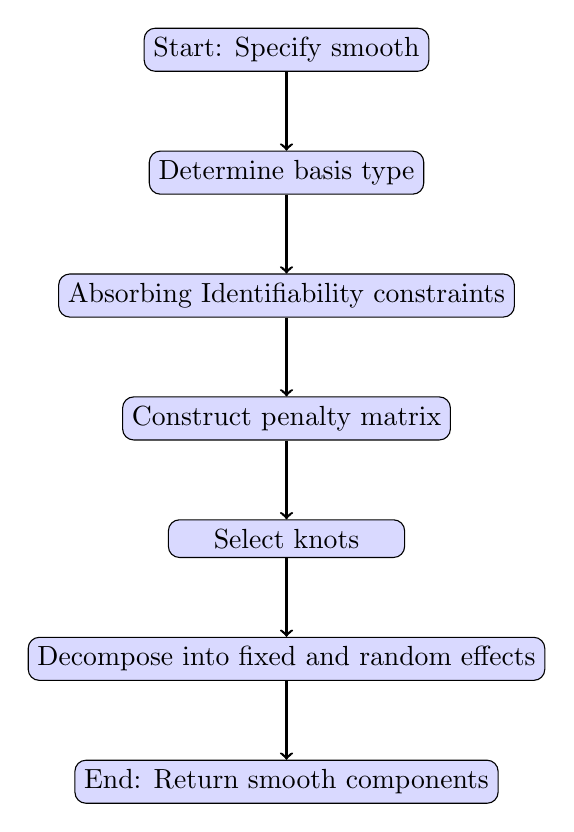
\begin{tikzpicture}[
    node distance=1cm,
    start chain=going below,
    every join/.style={->},
    every node/.style={draw, rounded corners, fill=blue!15, align=center, minimum width=3cm},
    arrow/.style={thick, ->}
]

% Nodes
\node (start) [on chain, join] {Start: Specify smooth};
\node (basis) [on chain, join] {Determine basis type};
\node (Absorb) [on chain, join] {Absorbing Identifiability constraints};
\node (penalty) [on chain, join] {Construct penalty matrix};
\node (knots) [on chain, join] {Select knots};
\node (decompose) [on chain, join] {Decompose into fixed and random effects};
\node (end) [on chain, join] {End: Return smooth components};

% Arrows
\draw [arrow] (start) -- (basis);
\draw [arrow] (basis) -- (Absorb);
\draw [arrow] (Absorb) -- (penalty);
\draw [arrow] (penalty) -- (knots);
\draw [arrow] (knots) -- (decompose);
\draw [arrow] (decompose) -- (end);

\end{tikzpicture}
\caption{Schematic overview of the \texttt{smoothCon} function from \texttt{mgcv}.}
\end{figure}


The \texttt{smoothCon} function in \texttt{mgcv} is a core utility designed to process smooth specifications in generalized additive models (GAMs). It essentially sets up the necessary matrices and information for representing and estimating the smooth components in the model. Here's an overview of its operation:

\begin{enumerate}[label=\arabic*., left=0pt]
    \item \textbf{Input Specification}: The function takes in a smooth specification, which typically consists of a combination of a predictor variable, a basis type (\texttt{bs} argument), and other options like the number of knots (\texttt{k} argument).
    
    \item \textbf{Determine Basis Type}: Based on the \texttt{bs} argument, \texttt{smoothCon} determines the type of basis functions to use. This choice influences the flexibility and shape of the smooth term. Common basis types include cubic splines (\texttt{cr}), thin plate splines (\texttt{tp}), and P-splines (\texttt{ps}), among others.

    \item \textbf{Absorbing Identifiability constraints}: \texttt{absorbs.cons=TRUE} ensures that the smooth terms are uniquely distinguishable and not confounded with other model components, like the intercept. The process employs QR decomposition, a mathematical method for transforming the basis functions such that they become orthogonal to the space of the constraints (e.g., the intercept). This orthogonality is essential because it prevents the overlap of effects between the smooth terms and the intercept, ensuring that each component of the model contributes distinctly to the explanation of the data. 

    
    \item \textbf{Construct Penalty Matrix}: One of the fundamental aspects of GAMs is the application of a penalty to the smooth terms to avoid overfitting. \texttt{smoothCon} constructs a penalty matrix appropriate for the chosen basis type. The penalty typically targets the "wiggly" parts of the smooth to ensure a balance between fit and smoothness.
    
    \item \textbf{Select Knots}: Knots are specific points in the data range where the spline functions can change direction. \texttt{smoothCon} selects appropriate knot locations based on the data and the specified number of knots (\texttt{k} argument).
    
    \item \textbf{Decompose into Fixed and Random Effects}: For certain applications, especially when using GAMs in mixed model frameworks, the smooth terms can be decomposed into fixed and random effects components. \texttt{smoothCon} provides the necessary decomposition, allowing the smooth to be used in packages like \texttt{gamm4}.
    
    \item \textbf{Output}: The function returns a list containing various components representing the smooth, including the basis functions, penalty matrices, and other relevant information.
\end{enumerate}


\subsection{Re-parametrizing Using smooth2random}

\begin{figure}[h]
\centering
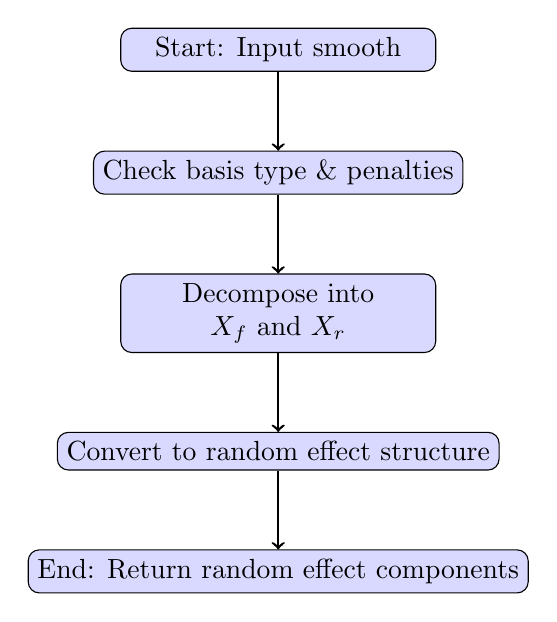
\begin{tikzpicture}[
    node distance=1cm, 
    start chain=going below,
    every join/.style={->},
    every node/.style={draw, rounded corners, fill=blue!15, align=center, minimum width=4cm},
    arrow/.style={thick, ->}
]

% Nodes
\node (start) [on chain] {Start: Input smooth};
\node (check) [on chain, join] {Check basis type \& penalties};
\node (decompose) [on chain, join] {Decompose into \\ \(X_f\) and \(X_r\)};
\node (convert) [on chain, join] {Convert to random effect structure};
\node (end) [on chain, join] {End: Return random effect components};

% Arrows
\draw [arrow] (start) -- (check);
\draw [arrow] (check) -- (decompose);
\draw [arrow] (decompose) -- (convert);
\draw [arrow] (convert) -- (end);

\end{tikzpicture}
\caption{Schematic overview of the \texttt{smooth2random} function from \texttt{mgcv}.}
\end{figure}

The \texttt{smooth2random} function in the \texttt{mgcv} package serves as a vital bridge between the realm of Generalized Additive Models (GAMs) and Generalized Linear Mixed Models (GLMMs). Its primary role is the transformation of smooth terms, typically utilized within GAMs, into a format that aligns with the structural requirements of random effects in GLMMs.

\begin{itemize}
    \item \textbf{Purpose}: The function's design facilitates the seamless integration of intricate spline-based effects into mixed models. This incorporation allows for the modeling of complex non-linear relationships, especially in scenarios with hierarchical or grouped data structures.
    
    \item \textbf{Functionality}: By converting smooth terms into random effect structures, \texttt{smooth2random} broadens the modeling capabilities, enabling researchers and analysts to capture and represent non-linear trends and patterns more effectively.
    
    \item \textbf{Impact}: The utility of \texttt{smooth2random} is especially pronounced in advanced modeling contexts, where the flexibility of GAMs is desired alongside the group-specific random effects of GLMMs.
\end{itemize}

In essence, \texttt{smooth2random} plays a pivotal role in expanding the horizons of mixed modeling, fusing the best of both GAMs and GLMMs to provide a robust toolset for statistical modeling.

\newpage




\subsection{How s() can be presented in \textbf{glmmTMB}}

While using the two functions we have mentioned above we can make the smoothing term in a \textbf{glmmTMB}-model.
\subsection*{R Code}

\begin{verbatim}
sm_tmpd <- mgcv::smoothCon(s(tmpd), absorb.cons = TRUE, 
                           data = chicago)[[1]]
                           
re_tmpd <- mgcv::smooth2random(sm_tmpd, "", type = 2)


Xf_tmpd <- re_tmpd$Xf
Xr_tmpd <- re_tmpd$rand[[1]]


chicago$ID <- factor(rep(1, nrow(chicago)))

ftmb1 <- glmmTMB(formula = death ~ Xf_tmpd +
                 homdiag(0 +Xr_tmpd | ID), 
                 data = chicago, REML=TRUE)
\end{verbatim}

\subsection*{Code Description}

\begin{enumerate}
    \item \textbf{Identifiability Constraints and Basis Function:}
    The code initializes a smooth term (\texttt{sm\_tmpd}) using \texttt{mgcv::smoothCon} with identifiability constraints absorbed into the basis, applicable to the variable \texttt{tmpd} in the \texttt{chicago} dataset.

    \item \textbf{Conversion to Random Effects:}
    The smooth term is then converted into random effects (\texttt{re\_tmpd}) using \texttt{mgcv::smooth2random}, specifying the type of conversion.

    \item \textbf{Extraction of Matrices:}
    Fixed effects matrix (\texttt{Xf\_tmpd}) and random effects matrix (\texttt{Xr\_tmpd}) are extracted from the converted smooth term.

    \item \textbf{Creating a Grouping Variable:}
    A fake grouping variable (\texttt{ID}) is created in the \texttt{chicago} dataset, assigning the same value to all observations for modeling purposes.

    \item \textbf{Generalized Linear Mixed Model (GLMM):}
    A GLMM (\texttt{ftmb1}) is fitted using \texttt{glmmTMB} to predict \texttt{death}, based on fixed effects and a random effect structure with a homogenous diagonal covariance structure, using Restricted Maximum Likelihood for estimation.
\end{enumerate}






\subsection{Basis functions in \textbf{glmmTMB}}



\begin{table}[h]
\centering
\caption{Compatibility of Spline Types in \texttt{glmmTMB}}
\begin{tabular}{lccc}
\toprule
Spline & bs & Compatible & Reasoning \\
\midrule
Cubic Regression & \texttt{"cr"} & \checkmark &  \\
Cyclical Cubic & \texttt{"cc"} & $\times$ & Only one Xf-term \\
Cubic Smoothing & \texttt{"cs"} & $\times$ &  No Xf-terms \\
Thin Plate Regression & \texttt{"tp"} & \checkmark &   \\
B-splines & \texttt{"bs"} &  \checkmark &  \\
P-splines & \texttt{"ps"} &  \checkmark &  \\
Two-dimensional Tensor Product & \texttt{"t2"} & \checkmark & \\
Two-dimensional Tensor Product & \texttt{"te"} & $\times$ & Not supported by smooth2random (gamm4) \\
Shrinkage Smooth & \texttt{"fs"}  & \checkmark & \\
Adaptive & \texttt{"ad"}  &$\times$ & Not supported by smooth2random  \\
Random Effect & \texttt{"re"}  & $\times$ & No Xf-terms \\
% Add other splines as needed
\bottomrule
\end{tabular}
\end{table}


\subsubsection{Proposition for\texttt{ bs="cs"} and \texttt{bs="cc"}}

The cyclical cubic spline and cubic spline does not have these Xf-terms, fixed effects, and the model will therefore not work with the code given is section 5.3. A seemingly nice alternative would be to code the model without the Xf-terms, as all the information from these basis funtions are given in the Xr-terms:

\begin{verbatim}
    ftmb1 <- glmmTMB(formula = death ~ 
    homdiag(0+Xr_tmpd | fake_group)
    , data = chicago, REML=TRUE)
\end{verbatim}

\subsection{Complexities of Tensor Product Splines}

Smooths of tensor product splines are more complicated and challenging to implement, due to their more complex construction and structure. One obstacle is handling the splitting of the prediction matrix into 4 matrices, three of which are Xr-matrices and one Xf-matrix. Understanding the finer details and mechanisms of how tensor product splines are constructed by the smooth constructor is crucial for managing their implementation in glmmTMB. 

\subsubsection{Tensor Product Splines in mgcv}


\subsection{Modeling convergence issues with s() in \textbf{glmmTMB}}

\begin{table}[H]
\centering
\begin{tabular}{>{\raggedright}p{4.5cm} >{\raggedright}p{6cm} >{\raggedright\arraybackslash}p{5.5cm}}
\toprule
\textbf{Model Convergence Issue} & \textbf{Description} & \textbf{Potential Solutions} \\
\midrule
Non-Positive-Definite Hessian Matrix & Occurs when the Hessian matrix at the solution is not positive definite, suggesting a non-unique solution or saddle point. & Check model specification, simplify the model, or provide better initial values. In cases where REML struggles to converge due to the model's complexity or data limitations, switching to ML might provide a more straightforward path to convergence. \\
\addlinespace
Iteration Limit or Objective Function Failure & Optimization algorithm didn't converge within iterations or failed to improve the objective function. & Increase iterations and evaluations, adjust CONVERGE value, or try different optimization methods. \\
\addlinespace
Inadequate Convergence or Local Minimum & Convergence criterion might only approximate a minimum point or converge to a local minimum. & Use different starting values, adjust convergence criteria, or employ a grid search for global minimum. \\
\addlinespace
Extreme Eigenvalues or False Convergence & Extreme eigenvalues suggest ill-conditioning, while false convergence indicates issues with gradient computation or tolerances. & Rescale data, check multicollinearity, restart the model with different starting values, or use alternative optimizers. \\
\addlinespace
Discontinuities or NA/NaN Evaluations & Discontinuities in the model or optimizer visiting invalid parameter spaces. & Ensure parameter estimates lie in a continuous interval, avoid discontinuity points, and ensure the optimizer leaves invalid regions. \\
\bottomrule
\end{tabular}
\caption{Common Convergence and Model-Fitting Issues in R for Non-Linear Models and GAMs}
\label{tab:model_convergence_combined}
\end{table}




\newpage

\section{compare}

\subsection{'Xr' Method: \(y \sim X_r\)}

In this method, we extract the random effect representation \(X_r\) of the smooth term and use it as a fixed effect in our model. Essentially, we are fitting the model:

\begin{equation}
y = X_r \beta + \epsilon
\end{equation}

Here, \(X_r\) is the design matrix for the smooth term, \(\beta\) is the vector of coefficients, and \(\epsilon\) is the error term.

\subsection{Ben Bolker's Method: \(y \sim (X_r | \text{dummy})\)}

Ben Bolker's approach integrates smooth terms directly into the \texttt{glmmTMB} package. The smooth term is represented in both the fixed and random effects part of the model. The model can be represented as:

\[
y = X_f \beta_f + Z \beta_r + \epsilon
\]

Here, \(y\) is the \(n \times 1\) response vector, \(X_f\) is the \(n \times q\) design matrix for the fixed effects, \(Z\) is the \(n \times m\) design matrix for the random effects (which includes the smooth terms), \(\beta_f\) is the \(q \times 1\) vector of fixed effect coefficients, \(\beta_r\) is the \(m \times 1\) vector of random effect coefficients, and \(\epsilon\) is the \(n \times 1\) error term.

The likelihood function is augmented with a penalty term \(P\):

\[
L(y | \beta_f, \beta_r) \propto e^{-\frac{1}{2} \beta_r^T S \beta_r}
\]

Here, \(S\) is the penalty matrix, which is used to smooth the curve.

we have a penalty matrix \(S\) and a basis function matrix \(B\). The smooth term can be represented as:

\[
s(x) = B \alpha
\]

Where \( \alpha \) is the vector of smooth coefficients. The penalty term for the smooth is:

\[
P = \alpha^T S \alpha
\]


e.g cubic splines, the penalty matrix \( S \) is typically a diagonal matrix with the first few diagonal elements set to zero. These zero elements correspond to the basis functions that make up the polynomial part of the spline (usually the intercept and the linear term). The remaining diagonal elements are positive and impose a penalty on the curvature of the spline.


\[
S = \begin{pmatrix}
0 & 0 & 0 & 0 \\
0 & 0 & 0 & 0 \\
0 & 0 & \lambda_1 & 0 \\
0 & 0 & 0 & \lambda_2
\end{pmatrix}
\]

Here, \( \lambda_1 \) and \( \lambda_2 \) are positive penalty terms.

In Bolker's method, the first two rows and columns from \( S \) are moved to the fixed effect model matrix \( X_f \). Because these rows and columns are zeros, moving them doesn't change the penalty imposed by \( S \). Instead, it changes how these terms are estimated:

- In the \( y \sim X_r \) method, these terms are estimated as fixed effects without any penalty.
- In the \( y \sim (X_r | \text{dummy}) \) method, these terms are estimated as fixed effects but are also subject to the penalty imposed by the random effects structure.
\newline

 Let's assume \(S_1\) represents these first two rows and columns, and \(S_2\) represents the remaining part of \(S\).

\[
S = \begin{pmatrix}
S_1 & 0 \\
0 & S_2
\end{pmatrix}
\]

The corresponding basis function matrix \(B\) can also be partitioned as \(B = [B_1, B_2]\), where \(B_1\) corresponds to \(S_1\) and \(B_2\) corresponds to \(S_2\).

The smooth term \(s(x)\) can then be partitioned as:

\[
s(x) = B_1 \alpha_1 + B_2 \alpha_2
\]

Here, \(\alpha_1\) would be treated as fixed effects and \(\alpha_2\) as random effects.


The GLMM is updated to:

\[
y = X_f \beta_f + B_1 \alpha_1 + Z \beta_r + B_2 \alpha_2 + \epsilon
\]

Here, \(B_1 \alpha_1\) is part of \(X_f\) and is estimated as fixed effects (\(\beta_f\)), while \(B_2 \alpha_2\) is part of \(Z\) and is estimated as random effects (\(\beta_r\)).


\subsection{Key Differences}

\begin{enumerate}
    \item \textbf{Intercept and Fixed Effects}: In Bolker's method, the first two rows and columns from the penalty matrix \(S\) are moved to the fixed effect model matrix. This essentially acts as an intercept. These terms are part of \(X_f\) and are estimated as fixed effects \(\beta_f\).
    
    \item \textbf{Random Effects}: The remaining part of the smooth term is included in the random effects matrix \(Z\), and its effects are estimated as random effects \(\gamma\).
    
    \item \textbf{Penalty Matrix}: The penalty matrix \(S\) is used to enforce smoothness, and its coefficients \(\theta\) are estimated in the model.
\end{enumerate}


\section{Penalization in Smooth Terms}

\subsection{Xr Method:}

In this approach, we are directly using the \(X_r\) terms as fixed effects without any explicit penalization. The \(X_r\) terms are essentially the basis functions that represent the smooth term. When you include them as fixed effects, they are not penalized, meaning that the model does not enforce any smoothness constraints on these terms. The model will fit these terms as it would any other fixed effect, aiming to minimize the residual sum of squares without any regularization.

Mathematically, the objective function looks something like:

\begin{equation}
\text{minimize} \quad ||y - X_r \beta||^2
\end{equation}

\subsection{Ben Bolker's Method:}

In Bolker's method, the smooth terms are included as both fixed and random effects, and they are subject to penalization through the penalty matrix \(S\). The penalty matrix \(S\) is used to enforce smoothness in the estimated function. The objective function in this case would include a penalty term:

\begin{equation}
\text{minimize} \quad ||y - X_f \beta_f - Z \gamma - S \theta||^2 + \lambda \theta^T S \theta
\end{equation}

Here, \(\lambda\) is the smoothing parameter, and \(S\) is the penalty matrix. The term \(\theta^T S \theta\) is the penalty term that enforces smoothness. The model aims to minimize this objective function, balancing the fit to the data and the smoothness of the estimated function.

\subsection{Key Differences in Penalization}

\begin{enumerate}
    \item \textbf{Explicit vs. Implicit Penalization}: Xr method does not include any explicit penalization, while Bolker's method includes a penalty term to enforce smoothness.
    
    \item \textbf{Objective Function}: The objective function in the Xr method aims to minimize the residual sum of squares, while Bolker's method aims to minimize a penalized residual sum of squares.
    
    \item \textbf{Smoothing Parameter}: In Ben Bolker's method, the smoothing parameter \(\lambda\) controls the trade-off between fit and smoothness, which is not present in the Xr method.
\end{enumerate}

\subsection{Summary}

In summary, the \(X_r\) terms in Xr method are essentially unpenalized, while in Bolker's method, the smooth terms are subject to penalization to enforce smoothness.

Now let's compare the \textbf{Xr} terms to the \textbf{s()} terms by looking at their structure. We will present the \textbf{Xr} term slightly differently here in order to make comparisons a bit easier to undertstand. 
\newline

The \(Xr\) terms in the `gtmb0` model are essentially basis function expansions that have been transformed into random effects. The model formula for `gtmb0` is:

\[
\text{death} \sim Xr_{\text{tmpd}} + Xr_{\text{time}} + Xr_{\text{pm10}} + Xr_{\text{pm25}}
\]

Each \(Xr\) term can be mathematically represented as:

\[
Xr_{\text{cov}} = \sum_{i=1}^{n} \beta_i B_i(x)
\]

Where:
- \( \beta_i \) are the coefficients.
- \( B_i(x) \) are the basis functions.
- \( n \) is the number of basis functions.
\newline

The \(s()\) terms in the `mgcv` model are smooth terms represented by penalized splines. The model formula for the `mgcv` model is:

\[
\text{death} \sim + s(\text{pm10median}) + s(\text{pm25median}) + s(\text{time}) + s(\text{tmpd})
\]

Each \(s()\) term can be mathematically represented as:

\[
s(x) = \sum_{i=1}^{n} \alpha_i B_i(x) + \lambda \int [s''(x)]^2 dx
\]

Where:
- \( \alpha_i \) are the coefficients.
- \( B_i(x) \) are the basis functions.
- \( n \) is the number of basis functions.
- \( \lambda \) is the smoothing parameter.

\subsection{Comparison}

\subsubsection{Smoothing Parameter in $s()$ Terms}

In the \(s()\) terms, the smoothing parameter \(\lambda\) explicitly controls the trade-off between the fit and the smoothness of the curve. Mathematically, the penalty term is:

\[
\lambda \int [s''(x)]^2 dx
\]

This term is added to the likelihood function, and its value is optimized during the model fitting process. A larger \(\lambda\) results in a smoother curve, while a smaller \(\lambda\) allows for more wiggly fits.

\subsubsection{Variance Structure in \(Xr\) Terms}

In the \(Xr\) terms, the smoothness is implicitly controlled by the random effects structure. Specifically, the random effects are assumed to follow a multivariate normal distribution with a certain covariance matrix \(\Sigma\):

\[
Xr_{\text{cov}} \sim \mathcal{N}(0, \Sigma)
\]

The elements of \(\Sigma\) can be considered analogous to the smoothing parameter in \(s()\) terms. They control the amount of "wiggle" allowed in the fitted curve. During the model fitting process, the elements of \(\Sigma\) are estimated from the data, effectively determining the smoothness of the \(Xr\) terms.

\subsubsection{Comparison and Equivalence}

\textbf{Implicit vs. Explicit Control:} \(s()\) terms have an explicit smoothing parameter \(\lambda\), while \(Xr\) terms have an implicit control through the random effects' covariance structure.
\newline

\textbf{Optimization:} Both \(\lambda\) and \(\Sigma\) are estimated during the model fitting process, albeit through different algorithms.
\newline

\textbf{Predictive Equivalence:} When both models are well-calibrated, the \(Xr\) terms in \texttt{gtmb0} and the \(s()\) terms in \texttt{gamm\_model} should produce similar predictions. This is because both are designed to capture the same underlying smooth relationship between predictors and response.
\newline

\textbf{Model Complexity:} The \texttt{gtmb0} model can be computationally less expensive because it fits within the generalized linear mixed model (GLMM) framework, which is well-optimized. On the other hand, \textbf{gamm\_model} may require specialized algorithms to optimize the smoothing parameter.

In summary, while the mechanisms are different, both \(Xr\) and \(s()\) terms aim to achieve similar goals of capturing the underlying smooth structure in the data. The \(Xr\) terms' random effects structure serves a role similar to the smoothing parameter in \(s()\) terms, making \texttt{gtmb0} and \textbf{gamm\_model} approximately equivalent in terms of their predictive capabilities.

\section{Domains for Spline Regression Application}

While spline regression models find applicability across a diverse array of phenomena, ranging from biological sciences to engineering, our focus on financial time series, insurance data, and large weather data is rooted in their particular relevance to the field of actuarial science. This selection aligns closely with the core areas of actuarial expertise, which include financial modeling, risk assessment, and quantitative analysis. Financial time series data is pivotal in understanding market dynamics and risk, essential for financial planning and investment strategies. Insurance data is at the heart of actuarial science, where accurate risk modeling is key to premium setting and risk management. Lastly, large weather data is increasingly crucial in actuarial work, especially considering the growing impact of climate change on risk calculations and insurance models. These domains not only provide a rich context for applying spline regression models but also are highly pertinent to the evolving role of actuaries in a world where data-driven decision-making is paramount.


\subsection{Financial Time Series Data}
In the realm of financial markets, characterized by inherent volatility and complex, non-linear dynamics, spline regression emerges as a particularly potent tool. It adeptly captures the intricate patterns observed in stock prices, interest rates, and market indices, accommodating for the frequent shifts and trends triggered by economic events, policy changes, and market sentiments. The flexibility of spline models in adapting to these abrupt fluctuations makes them invaluable for forecasting market movements, optimizing risk management, and identifying lucrative trading opportunities.

\subsubsection{Time Series Analysis}

We'll start off with some theory on time series analysis. In financial contexts it involves several critical considerations to accurately capture and predict complex temporal dynamics. Key concepts and methodologies are outlined below to guide this analytical process.
\newline

\subsubsection*{Definition of Auto-Correlation}

Auto-correlation, also known as serial correlation, refers to the correlation of a time series with its own past and future values. Mathematically, the auto-correlation function \(ACF\) for a time series \( \{X_t\} \) is defined as:

\[
ACF(\tau) = \frac{\text{Cov}(X_t, X_{t-\tau})}{\sqrt{\text{Var}(X_t) \times \text{Var}(X_{t-\tau})}}
\]

where \( \tau \) is the time lag, and \( \text{Cov} \) and \( \text{Var} \) are the covariance and variance, respectively.

\subsubsection*{Prevalence in Financial Time Series Data}

Auto-correlation is particularly prevalent in financial time series data for several reasons:

\begin{itemize}
    \item \textbf{Market Trends}: Financial markets often exhibit trends that persist over time, leading to positive auto-correlation.
    \item \textbf{Seasonality}: Many financial instruments show seasonal patterns, such as increased retail stock prices before holidays, which introduce auto-correlation.
    \item \textbf{Liquidity Constraints}: Trading restrictions or liquidity constraints can delay trading actions, causing a lagged effect and thus auto-correlation.
    \item \textbf{Information Diffusion}: Information takes time to propagate among market participants, leading to a gradual adjustment of prices and hence auto-correlation.
\end{itemize}

\subsubsection*{Implications}

The presence of auto-correlation in financial time series data has important implications:

\begin{itemize}
    \item \textbf{Modeling}: Traditional models like ordinary least squares (OLS) regression assume no auto-correlation; thus, specialized models like ARIMA or GARCH may be more appropriate.
    \item \textbf{Risk Assessment}: Auto-correlation can affect the volatility and predictability of financial instruments, impacting risk assessments.
    \item \textbf{Trading Strategies}: Understanding auto-correlation can help in developing more effective trading strategies, such as momentum or mean-reversion strategies.
\end{itemize}

\subsubsection*{Detection and Treatment}

Auto-correlation is commonly detected using statistical tests like the Durbin-Watson test or by examining the ACF and Partial Auto-Correlation Function (PACF) plots. Once detected, it can be treated or modeled using techniques like differencing, or by using models that explicitly account for auto-correlation, such as ARIMA or GARCH models.


\begin{itemize}
  \item Differencing: Transforming the series to a stationary one by differencing data points with their previous values.
  \item ARIMA models: Integrating autoregressive (AR) and moving average (MA) components to model the time series effectively.
  \item Lagged variables: Including past values as predictors in the regression model.
\end{itemize}




\subsubsection*{Overview of ARIMA Models}

ARIMA, which stands for AutoRegressive Integrated Moving Average, is a class of models that captures a suite of different standard temporal structures in time series data. The model is generally denoted as \(ARIMA(p, d, q)\), where:

\begin{itemize}
    \item \(p\) is the order of the AutoRegressive (AR) term,
    \item \(d\) is the number of differencing required to make the time series stationary,
    \item \(q\) is the order of the Moving Average (MA) term.
\end{itemize}

Mathematically, the ARIMA model can be expressed as:

\[
\phi(B)(1-B)^d X_t = \theta(B)Z_t
\]

where \( \phi(B) \) and \( \theta(B) \) are the AR and MA polynomials in the backshift operator \( B \), \( X_t \) is the time series, and \( Z_t \) is white noise.

\subsubsection*{Relevance in Financial Time Series Data}

ARIMA models are particularly useful in financial time series for several reasons:

\begin{itemize}
    \item \textbf{Flexibility}: The ARIMA model can capture a wide range of time series behaviors, including trends, seasonality, and auto-correlation, which are common in financial data.
    \item \textbf{Forecasting}: ARIMA models are widely used for short-term price and volatility forecasting.
    \item \textbf{Anomaly Detection}: The residuals from a well-fitted ARIMA model can be used to identify anomalies or outliers in financial data.
\end{itemize}


\subsubsection*{Preserving the Temporal Structure During Analysis}
The integrity of time series data is intrinsically tied to its temporal structure, which records the sequential interdependence of observations. Maintaining this order is pivotal when modeling financial time series, where patterns and trends across time are of primary interest. We will deploy several appropriate techniques to ensure the temporal structure is maintained.



\subsection{Modelling Log-Returns Post-COVID-19 and the Rise of Meme Stocks}

The onset of the COVID-19 pandemic introduced a period of very high volatility in global financial markets. Traditional linear models faced challenges in capturing these complex dynamics, particularly in the years 2020 and 2021. This period was also marked by the emergence of "meme stocks," such as GameStop and AMC Entertainment Holdings. These stocks experienced dramatic increases in value, driven by retail investors influenced by social media and trading platforms like Robinhood and Webull \cite{reuters2021meme}. However, the trend was characterized by extreme fluctuations, with some stocks trading significantly below their peak values \cite{reuters2021meme2}. The increased use of options trading further exacerbated market swings \cite{reuters2021options}.
\newline
    
Spline regression, known for its flexibility in accommodating abrupt changes and non-linear trends, may emerge as a more suitable analytical tool in this context. It can offer deeper insights into the post-COVID-19 financial landscape and aided in the development of robust forecasting and risk management strategies during these turbulent times.
\newline

\begin{center}
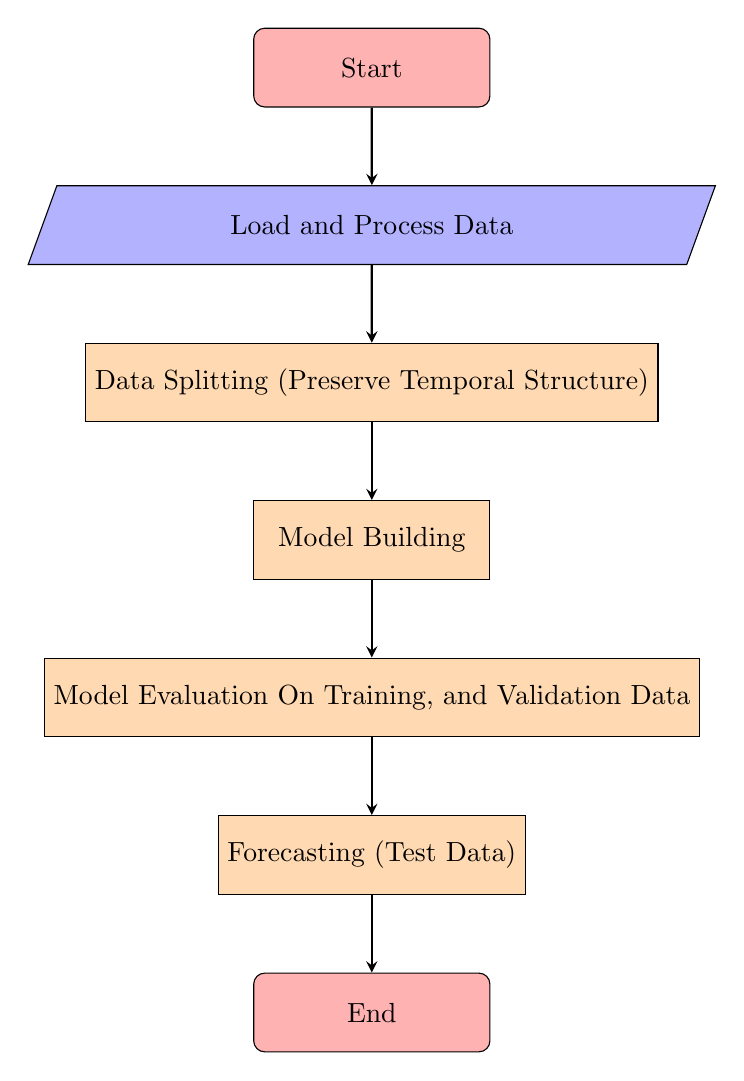
\begin{tikzpicture}[node distance=2cm]
\node (start) [startstop] {Start};
\node (data) [io, below of=start] {Load and Process Data};
\node (split) [process, below of=data] {Data Splitting (Preserve Temporal Structure)};
\node (model) [process, below of=split] {Model Building};
\node (evaluate) [process, below of=model] {Model Evaluation On Training, and Validation Data};
\node (forecast) [process, below of=evaluate] {Forecasting (Test Data)};
\node (end) [startstop, below of=forecast] {End};

\draw [arrow] (start) -- (data);
\draw [arrow] (data) -- (split);
\draw [arrow] (split) -- (model);
\draw [arrow] (model) -- (evaluate);
\draw [arrow] (evaluate) -- (forecast);
\draw [arrow] (forecast) -- (end);
\end{tikzpicture}
\end{center}

This figure illustrates the sequential steps involved in our time series regression analysis, highlighting the importance of data order preservation, model building with autocorrelation handling and non-linear modeling techniques, and thorough model evaluation before proceeding to forecasting.



\subsubsection{Analysis of the Model}

In this analysis, we focus on fitting three distinct models, but of the same form, using the \texttt{glmmTMB} package, each employing a different technique to approach spline regression. For the specific example demonstrated here, models of the form \texttt{log\_return $\sim$ s(time) + s(volume) + arima\_residuals, family = gaussian} were fitted, where the smooth terms in all models \textbf{TPRS} with \textbf{k = 10}. Bolker's method is more restricted in it's ability use other spline types (varying the bs=$"\cdot"$ parameter) than the other models, which are only constrained by the compatibility with \textbf{smooth2random}. The primary objective is to investigate key aspects such as efficiency, accuracy, and generalizability across these models.
\newline

The first model, referred to as \texttt{tmb1}, is a spline regression model that exclusively fits the "random part" — specifically, the matrix of basis functions denoted as \texttt{Xr}. In this model, these basis functions are estimated as fixed effects, with a manually implemented ridge penalty applied to regularize the model. This approach is expected to balance the model's flexibility with its ability to prevent overfitting, while being computationnaly efficient.
\newline

The second model, \texttt{tmb2}, mirrors \texttt{tmb1} in its form and structure. However, it distinctly lacks explicit regularization, meaning it does not include a ridge penalty. The comparison between \texttt{tmb1} and \texttt{tmb2} will provide insights into the impact of regularization on model performance, particularly in terms of accuracy and the risk of overfitting.
\newline

Finally, \texttt{tmb3} adopts the spline regression using Ben Bolker's version of a Generalized Additive Model (GAM) within \texttt{glmmTMB}. This model's implementation provides a more involved and sophisticated approach to spline fitting, but at the cost of computational efficiency. It will be serve as a comparison/benchmark. 


\subsubsection*{Data Preparation and Exploration}
Our program begins with data loading and preprocessing. Financial time series data, inherently non-linear and volatile, is loaded and prepared for analysis. This phase includes generating smooth terms and calculating ARIMA residuals, to enable effective spline modeling. 
\newline

\subsubsection*{Data Splitting Techniques}
We have meticulously ensured that the chronological sequence remains unaltered during data splitting for training, validation, and testing phases. Zero random sampling has been used in splitting data, only sequential cuts. We employed techniques such as rolling windows for cross-validation to preserve the contiguous nature of the data, thereby avoiding lookahead bias which can occur if future information is inadvertently incorporated into the model training process. Additionally, the residuals from the ARIMA models were used to account for autocorrelation within the time series, ensuring that the models capture the dependencies inherent in the data without being misled by spurious correlations. These measures collectively help safeguard the temporal structure, thus ensuring the reliability and validity of our model's predictions.

\subsubsection*{Ridge Penalty and Model Configuration}
A pivotal aspect of the program is the application of a ridge penalty in the spline regression model of interest. This regularization technique is crucial for managing the complexity of the models, avoiding overfitting, and enhancing predictive accuracy. Cross-validation is employed to determine the optimal lambda, the regularization parameter, ensuring the models strike a balance between flexibility and generalizability. Manually implementing the ridge penalty requires careful data augmentation which is described within the R-script. 

\subsubsection*{Model Fitting and Evaluation}
Three spline regression models are fitted on the prepared data — tmb1 with a ridge penalty, tmb2 as an unpenalized counterpart, and tmb3, a more sophisticated variant. Each model undergoes rigorous evaluation, including in-sample and cross-validation RMSE calculations, to assess predictive performance.
\newline

The three models will be assessed based on their computational efficiency (time taken for model fitting), accuracy (how closely the models predict the observed data), and generalizability (ability to perform well on unseen data, thus indicating resistance to overfitting). Through this comparative analysis, we aim to delineate the strengths and limitations of each modeling approach within the context of spline regression in financial time series data.


\subsubsection*{Advanced Model Analysis}
Beyond basic evaluations, the program delves into deeper analysis and diagnostics. This includes residual analysis, learning curve evaluation, and various statistical tests to comprehensively understand model behavior and effectiveness.


\subsubsection*{Visualization and Interpretation}
The program emphasizes the importance of visualization in interpreting model results. Plots and graphical representations are generated for RMSE trends, residuals, learning curves, and predicted versus actual values, facilitating an intuitive understanding of model performance.

\subsection{Comparing and Interpreting the Results}


\subsubsection*{In-Sample and Training}


\begin{table}[h]
\centering
\begin{tabular}{|l|c|c|c|c|}
\hline
Model & In-Sample RMSE & Time (sec) & AIC & BIC \\
\hline
tmb1 & 0.03034 & 0.4472 & -2689.85 & -2604.56 \\
tmb2 & 0.03100 & 0.4283 & -2675.70 & -2590.63 \\
tmb3 & 0.03033 & 1.2957 & -2655.41 & -2624.08 \\
\hline
\end{tabular}
\caption{In-sample RMSE, Model Fitting Time, AIC, and BIC on Training Data}
\end{table}


\subsubsection*{Test Data}
\newpage

\begin{figure}[ht!]
    \centering
    \begin{subfigure}[b]{0.45\textwidth}
        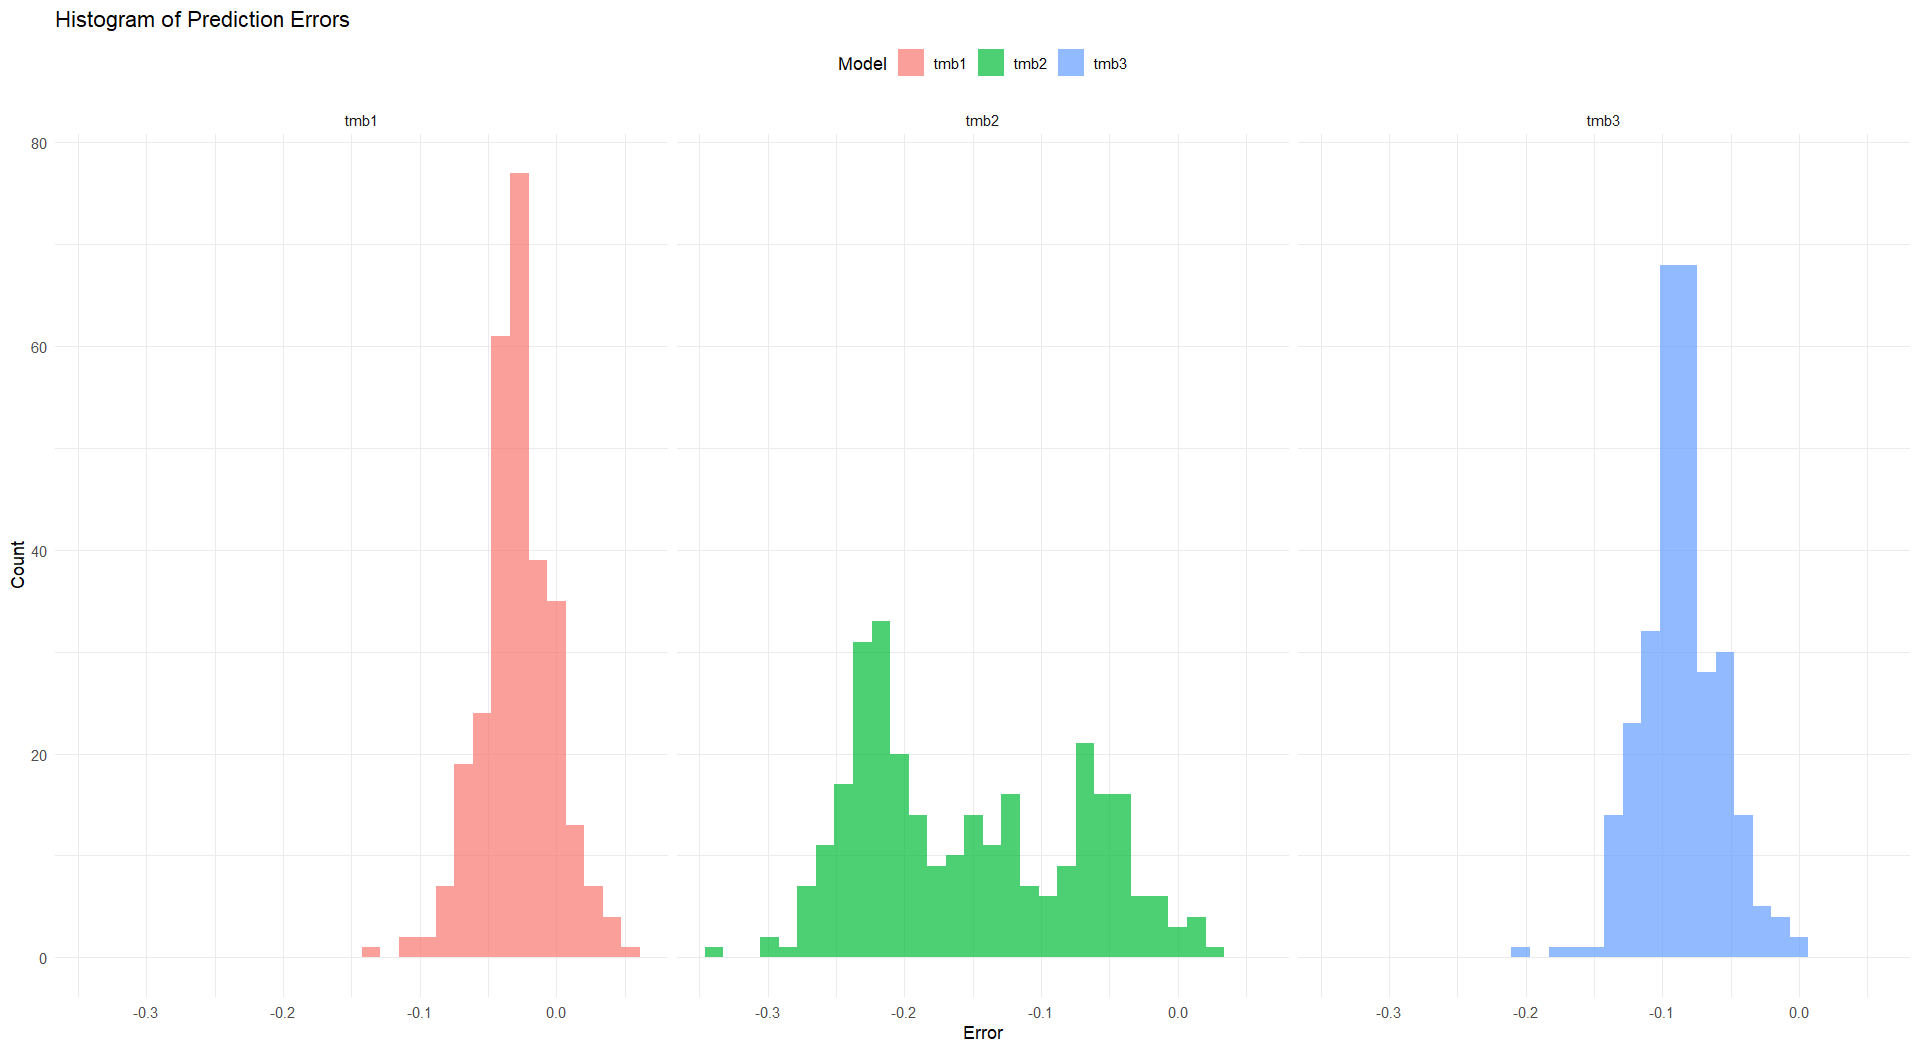
\includegraphics[width=\textwidth]{visuals/Visuals_ts_ridge/hist_pred_errors.png}
        \caption{Histogram of Prediction Errors}
        \label{fig:hist_pred_errors}
    \end{subfigure}
    \hfill
    \begin{subfigure}[b]{0.45\textwidth}
        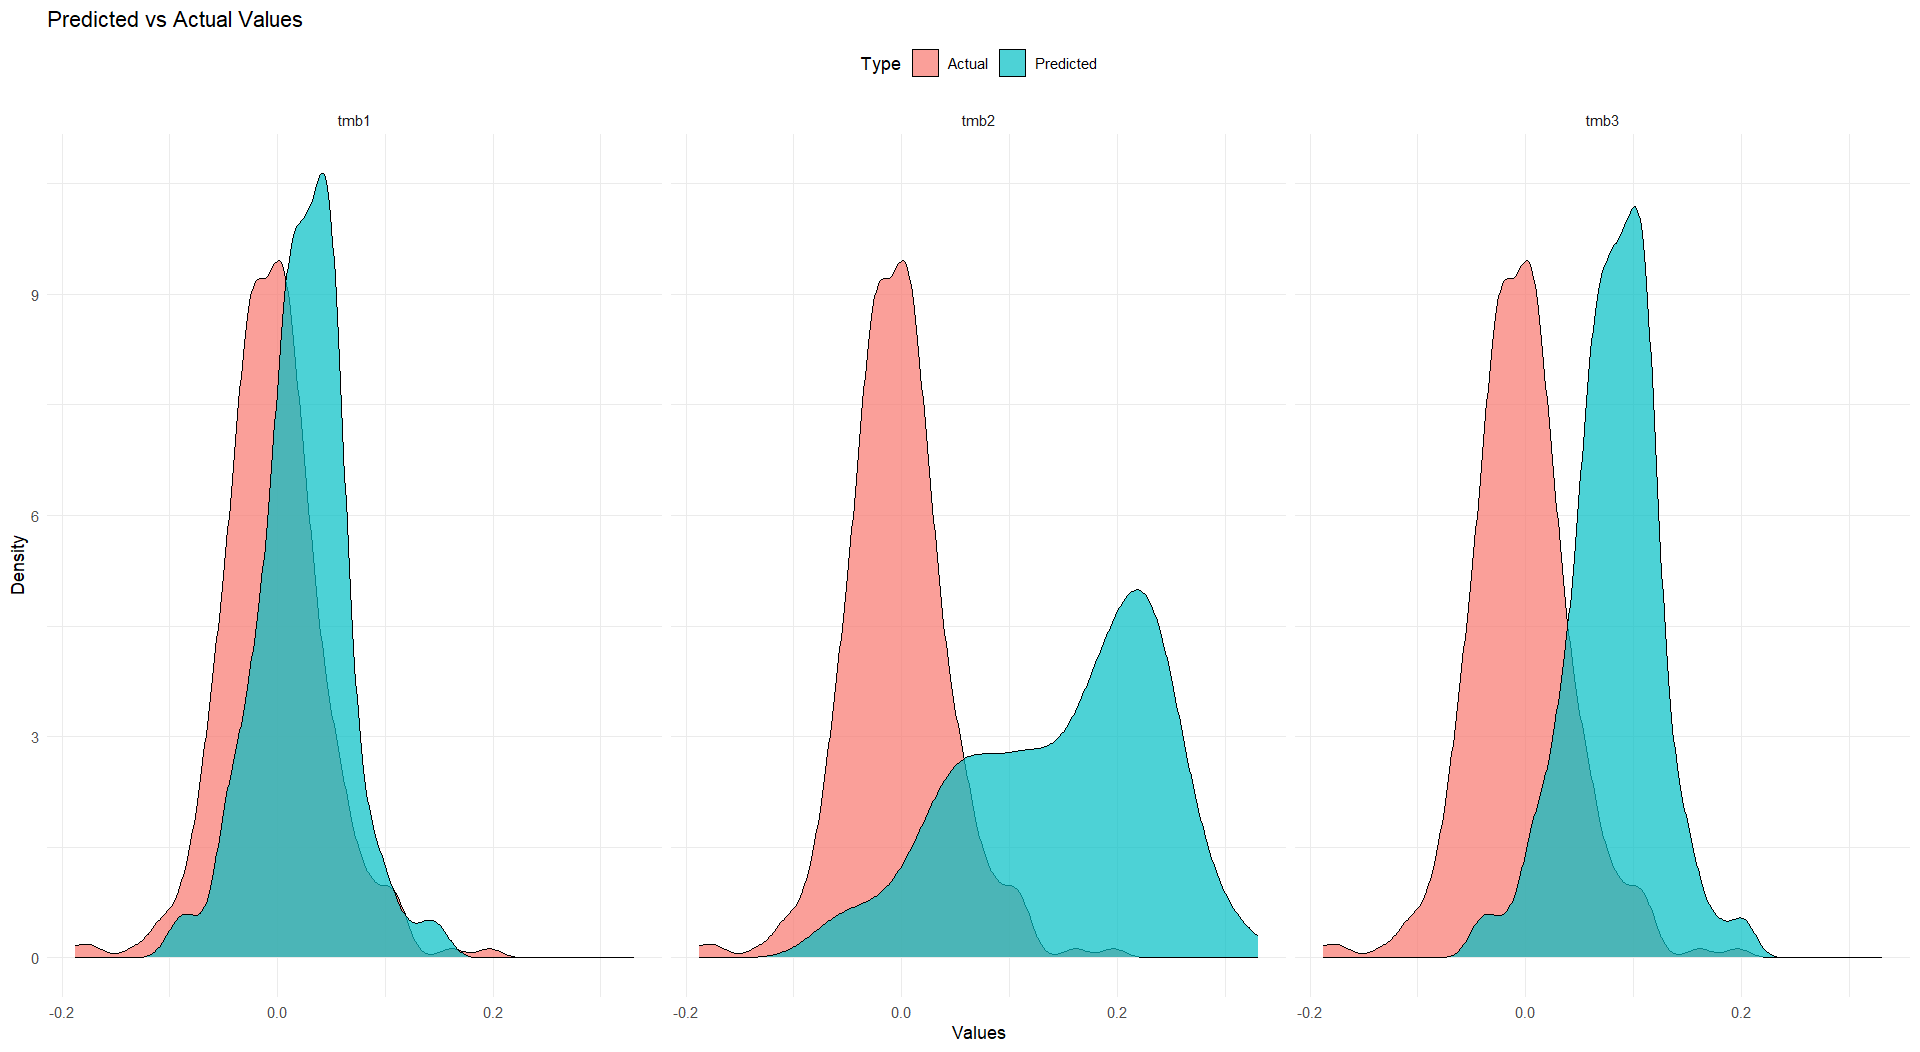
\includegraphics[width=\textwidth]{visuals/Visuals_ts_ridge/Predicted_vs_actual_densities_ts_ridge.png}
        \caption{Predicted vs Actual Densities}
        \label{fig:predicted_vs_actual_densities}
    \end{subfigure}
    \caption{Test Data Performance: Error Distribution and Density Comparison}
    \label{fig:test_data_performance_1}
\end{figure}


\begin{figure}[ht!]
    \centering
    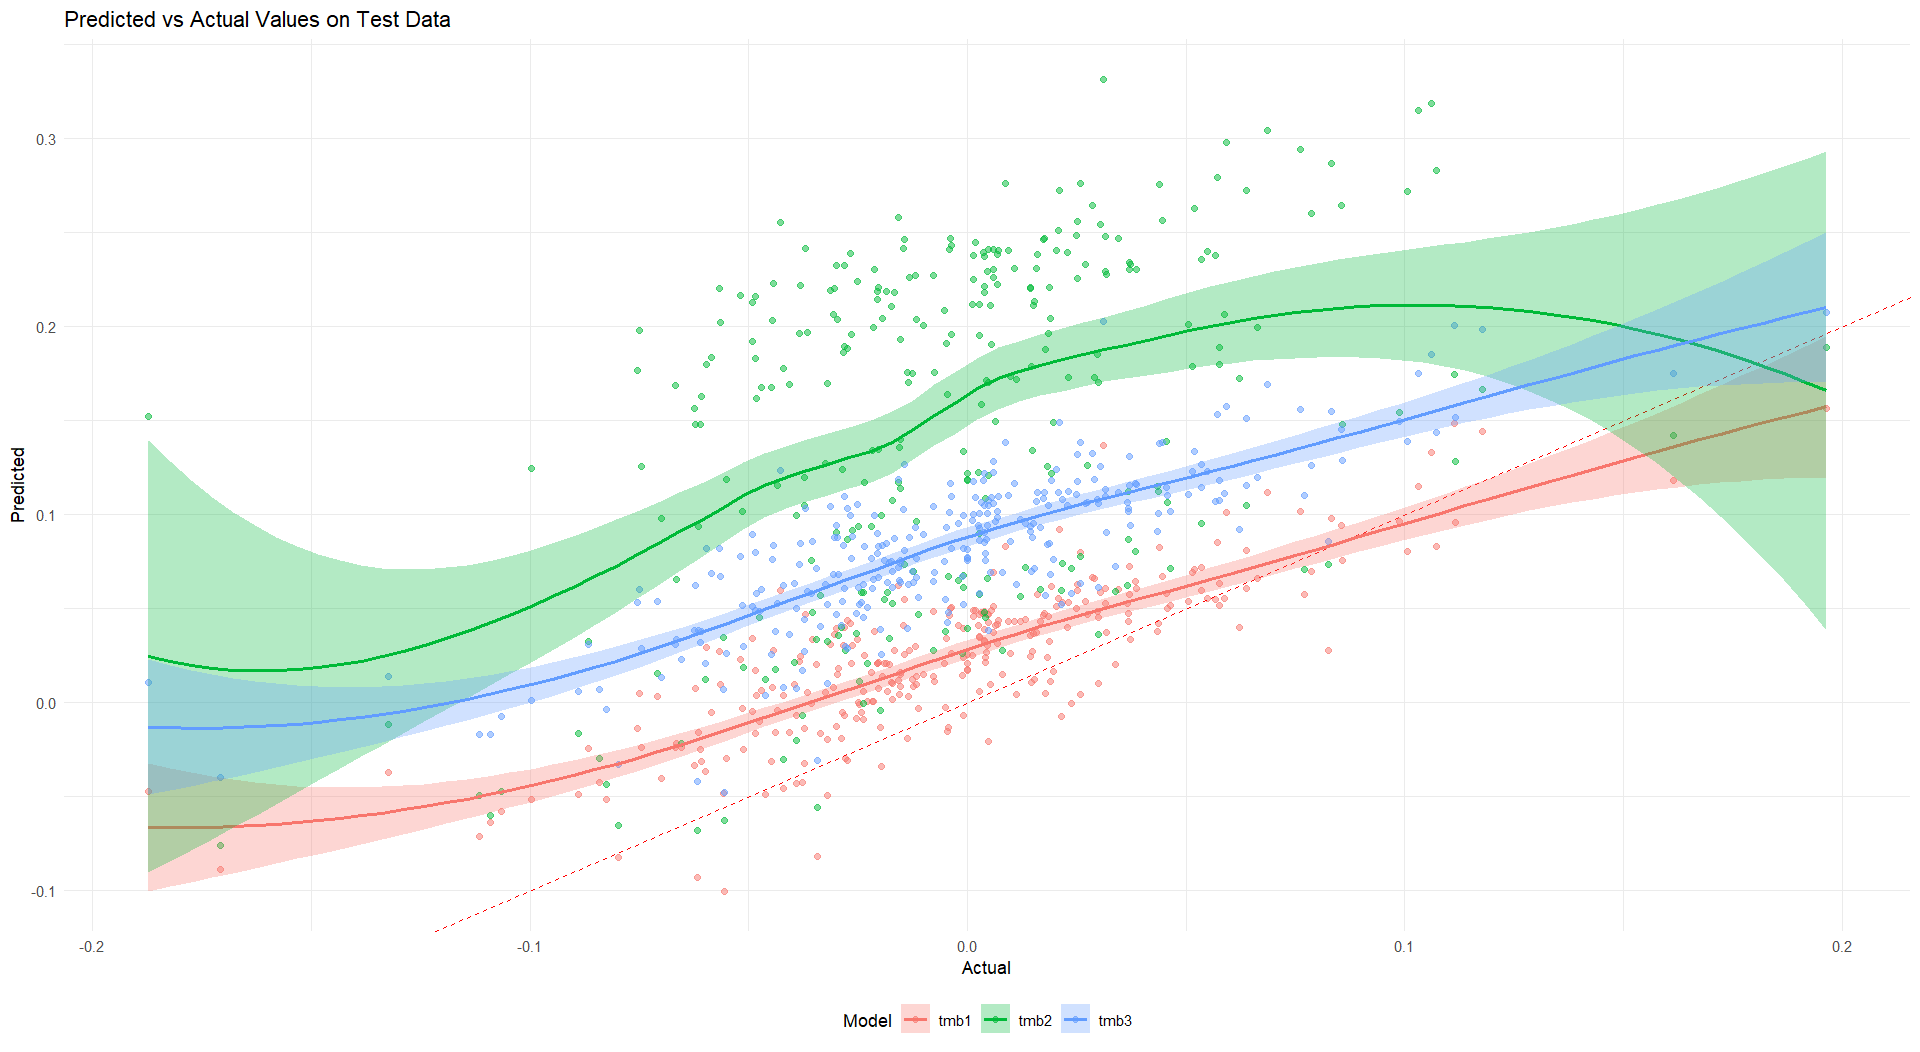
\includegraphics[width=0.9\textwidth]{visuals/Visuals_ts_ridge/predicted_vs_actual_test_data_lines.png}
    \caption{Predicted vs Actual Values with Loess Regression}
    \label{fig:predicted_vs_actual_lines}
\end{figure}


\begin{table}[h]
\centering
\begin{tabular}{|l|c|}
\hline
Model & RMSE on Test Data \\
\hline
tmb1 & 0.03912 \\
tmb2 & 0.17445 \\
tmb3 & 0.09075 \\
\hline
\end{tabular}
\caption{RMSE for Models on Test Data}
\end{table}


\subsection{Model Performance Summary}

\subsubsection*{Efficiency Analysis}
The computational efficiency of the models revealed a notable difference in time complexity. Models \texttt{tmb1} and \texttt{tmb2} exhibited similar computation times, approximately 3.79 and 3.66 seconds, respectively. Model \texttt{tmb3} required more substantial computational resources, with a total computation time of around 9.60 seconds, indicating the computational cost of the Generalized Additive Model (GAM) approach within \texttt{glmmTMB}.

\subsubsection*{In-Sample Performance}
The in-sample Root Mean Squared Error (RMSE) comparison showed that \texttt{tmb1} and \texttt{tmb3} performed similarly, whereas \texttt{tmb2} reported a marginally higher RMSE. This suggests that \texttt{tmb2} may not capture the training data's underlying patterns as effectively due to the absence of regularization.

\subsubsection*{Validation and Learning Curve Analysis}
Throughout the learning curve analysis, \texttt{tmb1} consistently outperformed the other models in terms of RMSE on the validation data, indicating a superior ability to generalize. Conversely, \texttt{tmb2} displayed highly variable RMSE values, particularly with smaller training sets, hinting at a propensity for overfitting. \texttt{tmb3} showed moderate RMSE values, suggesting better generalizability than \texttt{tmb2} but less so compared to \texttt{tmb1}.

\subsubsection*{Cross-Validation Metrics}
Across the cross-validation folds, \texttt{tmb1} achieved the best average metrics, including RMSE, Mean Absolute Error (MAE), and Mean Absolute Percentage Error (MAPE), corroborating its predictive accuracy. \texttt{tmb2} had the least favorable results, further suggesting overfitting. \texttt{tmb3} performed better than \texttt{tmb2} and exhibited the highest average R-squared, indicating a strong fit to the data's variance.

\subsubsection*{Test Data Evaluation}
On the unseen test data, \texttt{tmb1} maintained the lowest RMSE, reinforcing its robustness. \texttt{tmb2}'s performance on the test data was subpar, with a significantly higher RMSE, while \texttt{tmb3} provided a reasonable fit but was not as precise as \texttt{tmb1}.

\subsubsection*{Information Criteria Comparison}
The Akaike Information Criterion (AIC) and Bayesian Information Criterion (BIC) favored \texttt{tmb1}, with the lowest values indicating the best model considering both fit and complexity. \texttt{tmb3} did not offer a better fit to justify its computational cost, and \texttt{tmb2} was less efficient than \texttt{tmb1} when complexity was accounted for.


\subsubsection*{Conclusion}

In conclusion, \texttt{tmb1} surfaces as the most advantageous model for this particular dataset, striking an optimal balance between efficiency, accuracy, and generalization capabilities. The selection of the appropriate model may depend on the specific requirements of the analysis, and the specific financial time series dataset; however, \texttt{tmb1} would likely be a good choice in many scenarios.



\subsection{Insurance Data}
The insurance sector often grapples with non-linear risks influenced by diverse factors like age, health, lifestyle, and economic conditions. Spline regression models shine in this setting by enabling actuaries to predict claims with higher accuracy, set premiums more effectively, and understand nuanced risk factors. These models adeptly identify critical thresholds where risk levels undergo significant changes, thus playing a crucial role in refining policy pricing and formulating robust risk management strategies.




\begin{itemize}
    \item \textbf{Capturing Non-Linear Trends:} Insurance data, such as policy face values or customer age, often exhibit non-linear relationships. The \texttt{s()} function allows for flexible modeling of these relationships, fitting smooth, continuous curves that can better capture the underlying patterns in the data compared to traditional linear models.

    \item \textbf{Enhancing Model Accuracy:} By providing a more nuanced fit to the data, splines can improve the accuracy of predictive models. This is particularly important in insurance where predicting outcomes like policy uptake or claim probabilities accurately can significantly impact financial planning and risk assessment.

    \item \textbf{Interpretable Results:} While offering complexity, spline models remain interpretable. They allow actuaries and analysts to understand how different variables, such as age or income, non-linearly affect insurance variables like policy face amounts.

    \item \textbf{Flexibility:} The \texttt{s()} function allows for the specification of the degree of the spline and the number of knots, providing flexibility to the analyst in controlling the model's complexity. This adaptability is vital in dealing with diverse insurance datasets, which may require different levels of model flexibility.
\end{itemize}

Thus, the \texttt{s()} function is a powerful tool in the arsenal of any data analyst working with insurance data, offering a balance between flexibility, interpretability, and the ability to accurately model complex, non-linear relationships inherent in such data.



\subsubsection{Exploring the \textbf{ustermlife} data set}




\begin{figure}[ht!]
    \centering
    \begin{subfigure}[b]{0.45\textwidth}
        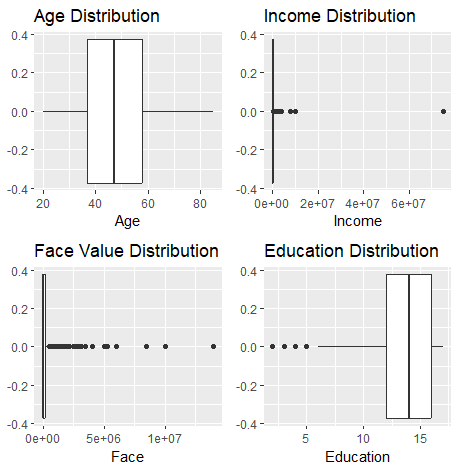
\includegraphics[width=\textwidth]{visuals/InsuranceVisuals/UstermHist.png}
        \caption{Histogram of variables}
        \label{fig:hist_of_variables}
    \end{subfigure}
    \hfill
    \begin{subfigure}[b]{0.45\textwidth}
        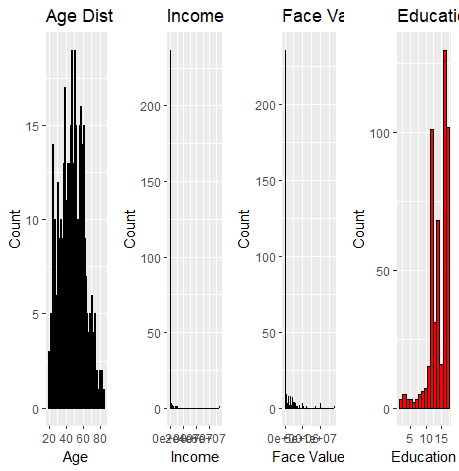
\includegraphics[width=\textwidth]{visuals/InsuranceVisuals/UstermDist.png}
        \caption{Distribution of variables}
        \label{fig:Distribution_of_variables}
    \end{subfigure}
    \caption{EDA of the data set}
    \label{fig:test_data_performance_1}
\end{figure}

\newpage
\begin{figure}[ht!]
    \centering
    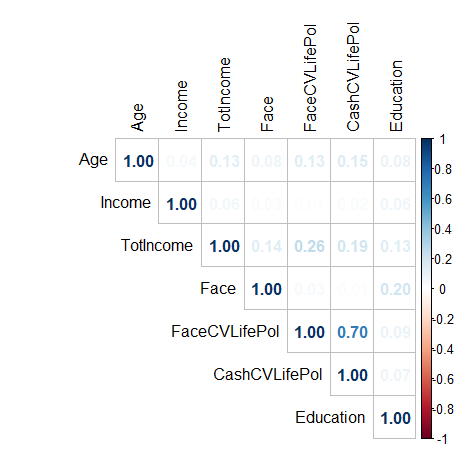
\includegraphics[width=0.9\textwidth]{visuals/InsuranceVisuals/UsTermCorr.png}
    \caption{Correlation matrix of the variables}
    \label{fig:cor_variables}
\end{figure}
\newpage
\begin{figure}[ht!]
    \centering
    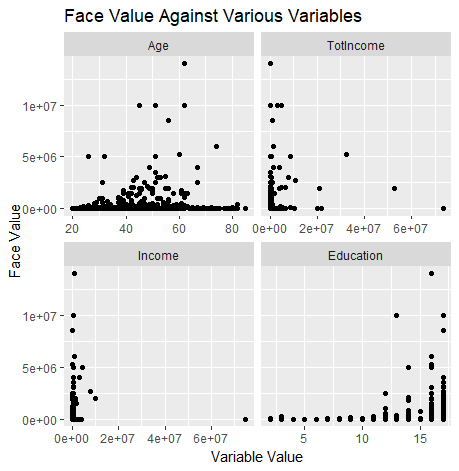
\includegraphics[width=0.9\textwidth]{visuals/InsuranceVisuals/FaceValueVcovariates.png}
    \caption{Plots of Face versus covariates}
    \label{fig:FaceVscovariates}
\end{figure}

\newpage
\begin{figure}[ht!]
    \centering
    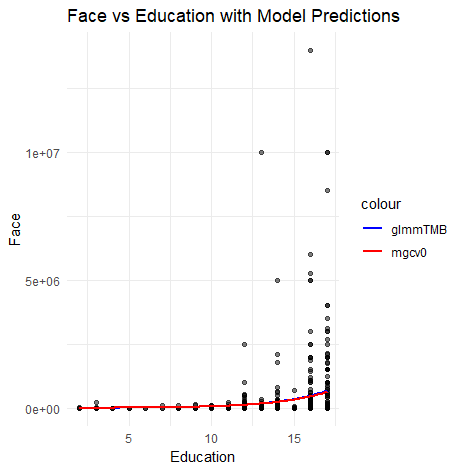
\includegraphics[width=0.9\textwidth]{visuals/InsuranceVisuals/FacevEducation.png}
    \caption{Plot of \textbf{glmmTMB} versus \textbf{mgcv}}
    \label{fig:FaceVseducation}
\end{figure}






\subsection{Ustermlife Dataset}
The \texttt{ustermlife} dataset is sourced from the Survey of Consumer Finances (SCF), representing a nationally representative sample of U.S. households. It includes data from 500 households with positive incomes, surveyed in the year 2004. The dataset provides a detailed snapshot of various aspects:

\begin{itemize}
    \item \textbf{Demographics:} It records demographic characteristics such as age, gender, education level, and marital status of the respondents and, where applicable, their spouses.
    \item \textbf{Financial Information:} The dataset includes comprehensive data on household assets, liabilities, annual income, and total income. This information offers insights into the financial health and capabilities of the sampled households.
    \item \textbf{Term Life Insurance:} A key focus of the dataset is on term life insurance. It measures the quantity of insurance through the policy face value - the amount payable by the insurance company in the event of the insured's death.
    \item \textbf{Household Composition:} Information about the number of members in each household is included, providing context to the financial and insurance data.
\end{itemize}


\subsubsection{Summary Statistics of the Ustermlife Dataset}
The \texttt{ustermlife} dataset, encompassing data from 500 households, provides insightful statistics across various demographic, financial, and insurance-related variables:

\begin{itemize}
    \item \textbf{Age:} The ages of respondents range from 0 to 78 years, with an average age of approximately 33.4 years, suggesting a diverse sample in terms of age groups.
    
    \item \textbf{Income and Total Income (TotIncome):} These financial metrics demonstrate a wide range, indicating significant variability in household economic statuses. The broad range highlights the diverse financial circumstances of the sampled households.
    
    \item \textbf{Face Value (Face):} The insured amounts vary substantially, ranging from policies with no coverage to those with a coverage of up to 14 million. This variation reflects the different levels of financial protection sought by the households.
    
    \item \textbf{Education:} Education levels among respondents vary from 0 to 17 years, providing insights into the educational diversity within the sample.
\end{itemize}

\subsubsection*{Distribution of Continuous Variables}
\begin{itemize}
    \item \textbf{Age:} The distribution of age appears to be fairly normal, indicating a balanced representation across different age groups within the sample.
    
    \item \textbf{Income-Related Variables:} Variables such as Income, Total Income, Face Value, Face Value of Life Insurance Policy with Cash Value (FaceCVLifePol), and Cash Value of Life Insurance Policy (CashCVLifePol) exhibit right-skewed distributions. This skewness is typical in income and wealth data, where a smaller proportion of high values extends the distribution's tail to the right, reflecting the presence of higher-income or higher-wealth households in the sample.
\end{itemize}





\subsubsection{Generalized Linear Model Analysis}
We conducted a Generalized Linear Model (GLM) analysis to explore the relationship between the Face Value of insurance policies and various demographic, financial, and policy-related factors. The model is defined as follows:

\begin{verbatim}
glm(formula = Face ~ Age + Gender +
Education + MarStat + Ethnicity + 
    SmarStat + Sgender + Sage + Seducation + 
    NumHH + Income + 
    TotIncome + Charity + FaceCVLifePol + CashCVLifePol + 
    BorrowCVLifePol + 
    NetValue, data = data)
\end{verbatim}

From the output of the model, the following covariates were found to be significant:

\begin{itemize}
    \item \textbf{Education}: The number of years of education of the survey respondent showed a positive relationship with the Face Value, with an estimated coefficient of \(4.802 \times 10^4\) (p-value = 0.0477).
    \item \textbf{Seducation}: The education level of the respondent's spouse also turned out to be significant, with an estimated coefficient of \(6.362 \times 10^4\) (p-value = 0.0227).
    \item \textbf{NumHH}: The number of household members was positively associated with the Face Value, with an estimated coefficient of \(1.042 \times 10^5\) (p-value = 0.0239).
    \item \textbf{TotIncome}: The total income of the household had a significant effect on the Face Value, with an estimated coefficient of \(2.988 \times 10^{-2}\) (p-value = 0.0195).
\end{itemize}

These results suggest that education, household size, and total income are significant predictors of the Face Value of a life insurance policy. The other covariates, including Age, Gender, Marital Status, and others, were not found to be significant in this model. 

\subsubsection*{stepAIC}

We can also use the step function in R that measures the different models AIC as a way of finding the best model. This function says that according to the AIC we should also include Gender and Age to the model so we proceed with the model:

\begin{verbatim}
    model0 <- glmmTMB(Face ~Age + Gender
    +NumHH+ Education+ 
    Sgender + Seducation
    +TotIncome, data=data)

summary(model0)
    
\end{verbatim}


\subsubsection{Introducing the Tweedie distribution}

As the Face values we encounter have a value of zero if they have not been claimed, and has more of a gamma distribution, it is fair to assume that a model using the tweedie-function in \textbf{glmmTMB} could be a good approach.
\newline

However when using tweedie, the large differences of value from TotalIncome is not accepted, so we make a new variable of the log of TotalIncome called \textit{TotalIncome\_log} so that our model looks like;

\begin{verbatim}
    model0 <- glmmTMB(Face ~Age+
    Gender+NumHH+ Education+ 
    Seducation+ TotIncome_log
    , data=data, family = tweedie())
    
\end{verbatim}

Comparing these two models we can see by the AIC that the tweedie model is a much better fit for this predictor;

\begin{table}[ht]
\centering
\caption{AIC Comparison of Models}
\begin{tabular}{lcc}
\hline
Model & Degrees of Freedom (df) & AIC \\
\hline
Gaussian & 9 & 15459.105 \\
Tweedie & 9 & 8356.823 \\
\hline
\end{tabular}
\label{tab:aic_comparison}
\end{table}







\newpage

\subsection{sgautonb Dataset}
The sgautonb dataset, encompassing automobile injury claim numbers in Singapore, offers a comprehensive view of factors influencing insurance claims. This subsection delves into the key variables and their potential impact on the number of claims (\textit{Clm\_Count}).

\begin{itemize}
    \item \textbf{SexInsured (Gender of Insured)}: Categorized as Male, Female, or Unspecified, this variable may reflect different risk profiles and driving behaviors, potentially influencing claim frequencies.
    
    \item \textbf{VehicleType}: Encompassing types such as Automobile, Truck, and Motorcycle, the variable could indicate varying levels of risk associated with different vehicle types, thereby affecting claim counts.
    
    \item \textbf{PC (Private Vehicle)}: This binary indicator of whether a vehicle is private might correlate with usage patterns, influencing the likelihood and frequency of claims.
    
    \item \textbf{NCD (No Claims Discount)}: Reflecting the policyholder's accident history, where higher discounts denote better records, NCD could be a strong predictor of future claim tendencies.
    
    \item \textbf{AgeCat (Age Category of Policyholder)}: Categorizing policyholders' ages, this variable is crucial in assessing risk, as different age groups may exhibit varied driving behaviors impacting claim frequency.
    
    \item \textbf{VAgeCat (Age Category of Vehicle)}: The age of vehicles, grouped categorically, could be significant, with older vehicles potentially having a higher propensity for claims due to increased breakdown risks.
    
    \item \textbf{Exp\_weights (Exposure Weight)}: Representing the policy duration as a fraction of the year, longer exposure periods could logically lead to a higher probability of filing claims.
\end{itemize}

To quantitatively assess the impact of these variables on claim counts, statistical methods such as descriptive analysis, correlation studies, and regression modeling (specifically Poisson or negative binomial regression) are recommended. These approaches, particularly regression analysis, can elucidate the extent to which each factor contributes to the likelihood and frequency of insurance claims. 



\subsection{Big Data}

The advent of "Big Data" has revolutionized the landscape of computational analysis and decision-making. Big Data refers to datasets that are so large or complex that traditional data processing applications are inadequate. The utility of Big Data lies in its ability to provide unprecedented insights and predictive power across various fields, from healthcare to finance. With the advancement of technologies such as machine learning and data mining, Big Data has become a cornerstone in driving innovations and efficiencies.
\newline

However, the complexity and challenges associated with Big Data cannot be understated. One of the primary concerns is the scalability of computational models as data size increases. The relationship between dataset size and computational complexity is often non-linear. As detailed in the research by Leskovec, Rajaraman, and Ullman (2014), the complexity of algorithms can scale superlinearly with data size, leading to exponentially increasing computational resource requirements and processing time.
\newline

Furthermore, the management and analysis of Big Data require significant computational resources, both in terms of hardware and software. As the size of the data grows, the time required for processing and analysis grows as well, often requiring parallel and distributed computing techniques to manage effectively. Empirical studies, such as those conducted by Dean and Ghemawat (2008) in the context of Google's MapReduce, demonstrate how distributed computing frameworks can manage and process large datasets, but also highlight the complexity and resource demands of such operations.
\newline

Another challenge in Big Data is ensuring data quality and integrity. The volume and variety of data often lead to inconsistencies, noise, and missing values, which can significantly affect the outcomes of data analysis. Addressing these issues requires additional preprocessing steps, further adding to the computational load.
\newline


\subsubsection{Challenges and Strategies in Modeling Large Datasets on Personal Computers}

Modeling large datasets on personal computers presents unique challenges due to the limitations of hardware resources and processing power. Unlike enterprise-level computational resources, personal computers have finite, often limited, capacities in terms of memory, storage, and processing capabilities. The complexity of computational models and the size of datasets typically scale non-linearly, which can have significant implications on hardware requirements and time usage.

\textbf{Non-Linear Scaling of Complexity}: Theoretical and empirical studies have shown that the computational complexity of algorithms used in data modeling often scales superlinearly with the size of the data. For instance, certain machine learning algorithms have a complexity of \( O(n^2) \) or even \( O(n^3) \), where \( n \) is the number of data points (Cormen et al., 2009). This non-linear scaling means that doubling the dataset size more than doubles the computational effort, leading to exponential increases in processing time and memory usage.

\textbf{Hardware Limitations}: On a typical modern personal computer, which may have between 4 to 16 cores, and in some state-of-the-art high-end models up to 96 cores, the challenge lies in efficiently utilizing these cores for parallel computation. The memory (RAM) is also a bottleneck; larger datasets require more memory, and once the available RAM is exceeded, the computer resorts to using slower disk-based storage, further impacting performance. A typical modern PC has 8-32GB of RAM, with very high end models having 64-128GB. 

\textbf{Strategies for Effective Modeling}:
\begin{itemize}
    \item \textit{Data Preprocessing}: Techniques such as dimensionality reduction, sampling, and data cleaning can significantly reduce the size of the dataset without substantial loss of information, making it more manageable for personal computers.
    \item \textit{Algorithm Optimization}: Choosing algorithms with lower complexity or optimizing existing algorithms to be more efficient can mitigate the effects of non-linear scaling. For example, using approximation algorithms or algorithms with linear time complexity can be more suitable for large datasets.
    \item \textit{Parallelization}: Utilizing the multi-core architecture of modern CPUs through parallelization can significantly reduce computation time. Techniques like multithreading or using parallel processing libraries allow for distributing the workload across multiple cores.
\end{itemize}

In conclusion, while modeling large datasets on personal computers is challenging due to hardware limitations and the non-linear scaling of model complexity, strategies like data preprocessing, algorithm optimization, and parallelization provide viable pathways to effectively manage and analyze large datasets.

\subsubsection{Parallelization and Optimization}

Parallelization in statistical models and computing represents a pivotal shift in the way data analysis is performed in a multi-core and distributed computing environment. Traditionally, computational tasks in statistics are performed sequentially, but parallelization breaks these tasks into smaller, independent sub-components that can be executed concurrently. This approach is particularly transformative in statistical modeling, where processes such as simulations, bootstrapping, or cross-validation are inherently repetitive and can be parallelized effectively.
\newline

The benefit of parallelization is most pronounced in the context of handling complex models and large datasets. For example, complex climate and weather models that use long running historical data, to model and predict non-linear relationships between continous variables. 
\newline

The rise of parallel computing has spurred the development of new statistical methodologies and software designed for parallel execution. This includes the integration of parallel processing capabilities in popular programming languages like R and Python, offering statisticians and data scientists the tools to implement parallelization with ease. However, parallelization also introduces challenges such as synchronization, managing data dependencies, and the overhead associated with task distribution and result integration. Nonetheless, the advantages of parallelization, especially in handling extensive data analyses and complex statistical models, are substantial, underscoring its essential role in contemporary statistical computing.

\subsubsection*{Parallelization in R using \texttt{furrr} and \texttt{future} Packages}

The implementation of parallelization in R has been greatly enhanced with the introduction of the \texttt{furrr} and \texttt{future} packages. These packages offer a streamlined approach to parallel computing, enabling R users to efficiently leverage the power of multi-core processors and distributed computing systems.
\newline

The \texttt{future} package in R provides a unifying framework for executing R expressions asynchronously. It allows for the abstraction of the details of parallel execution, enabling the user to write code without the need to consider the underlying complexities of parallel processing. This package supports various parallel backends, including multicore, multiprocess, and cluster options, providing flexibility in choosing the most suitable parallelization strategy for a given task.
\newline

Building on the capabilities of \texttt{future}, the \texttt{furrr} package extends the well-known \texttt{purrr} package's functional programming tools to a parallel setting. \texttt{furrr} enables the use of common \texttt{purrr} functions, such as \texttt{map} and \texttt{walk}, in parallel, by simply replacing them with their \texttt{future}-based counterparts, like \texttt{future\_map} and \texttt{future\_walk}. This seamless integration allows for easy adaptation of existing R code to utilize parallel computing, without the need for extensive rewrites.
\newline

The combination of \texttt{furrr} and \texttt{future} in R significantly simplifies the process of parallelizing code. Users can write more readable and maintainable code while harnessing the computational power of parallel processing. This is particularly useful for tasks that involve large-scale simulations, complex data manipulations, or computationally intensive algorithms, where the speedup gained from parallelization can be substantial.


\subsubsection*{Efficiency and Overhead in Parallelized k-Fold Cross-Validation}

To take present an example of the efficacy of parallelization, we will look at k-fold cross-validation. We can theoretically enhance computational efficiency significantly. Let us consider a k-fold cross-validation process parallelized across \( k \) processors. Ideally, if each fold is processed independently and simultaneously, the computational time \( T \) could theoretically be reduced by a factor close to \( k \), assuming perfect parallelization. This ideal speedup \( S \) can be represented as:

\[ S = \frac{1}{\left(1 - p\right) + \frac{p}{k}} \]

where \( p \) represents the parallelizable fraction of the task. In the case of k-fold cross-validation, \( p \) is approximately 1, as each fold is independently processed. This relation is derived from Amdahl's Law, which provides a theoretical limit on the maximum improvement to an overall system's processing speed when only part of the system is improved \cite{amdahl1967validity}.

However, practical implementations of parallelization often yield less than this theoretical maximum due to various overheads. These overheads include, but are not limited to, the time for data distribution (\( T_{\text{data}} \)), synchronization (\( T_{\text{sync}} \)), and inter-process communication (\( T_{\text{comm}} \)). Thus, the actual speedup \( S_{\text{actual}} \) is often represented as:

\[ S_{\text{actual}} = \frac{T}{T/k + T_{\text{data}} + T_{\text{sync}} + T_{\text{comm}}} \]

In distributed computing environments, particularly, \( T_{\text{comm}} \) can become a significant factor. The overheads are also influenced by the size of the dataset and the architecture of the computing environment \cite{gustafson1988reevaluating}.

Furthermore, the efficiency of parallelization is influenced by the law of diminishing returns, as described by Gustafson's Law, which suggests that increasing the number of processors will yield diminishing speedups due to the fixed size of the sequential portion of the task (Gustafson, 1988).

In summary, while parallelization in k-fold cross-validation can offer theoretical speed improvements, actual gains are moderated by the overheads associated with parallel process management and data communication. The balance between the theoretical speedup and the practical overheads determines the efficiency of parallelization in such computational tasks.

\subsubsection{Weather Data}

Weather patterns and climate phenomena, marked by their complexity and dynamism, require analytical approaches beyond linear modeling. Spline regression's flexibility makes it apt for modeling weather data, capturing non-linear interactions between various meteorological variables. This is particularly pivotal in climate research, weather forecasting, and understanding long-term climatic changes. Spline models are instrumental in analyzing trends in temperature, precipitation patterns, and other atmospheric conditions, thus contributing significantly to sectors like agriculture, disaster management, and environmental planning.

\subsubsection{Extending ARIMA Models}



\subsection{Modelling (insert response) from Large Weahter Data}


\subsubsection*{Dataset 1}


The Weather Anomalies dataset provides a comprehensive account of temperature deviations from historical averages, recorded by various weather stations from 1964 to 2013. This dataset is a hybrid collection, combining raw data from the National Oceanic and Atmospheric Administration (NOAA) with calculated figures based on Enigma's weather data.

\begin{itemize}
    \item \textbf{Date (date\_str):} Each entry in the dataset is timestamped, following a year-month-day format, which represents the date of the temperature recording.
    
    \item \textbf{Degrees from Mean (degrees\_from\_mean):} This column quantifies the deviation of the recorded temperature from the historical monthly average, providing insight into the extent of the temperature anomaly.
    
    \item \textbf{Station ID (id):} A unique identifier assigned to each weather station, facilitating data traceability and station-specific analyses.
    
    \item \textbf{Geographic Coordinates:} The dataset includes longitude and latitude information for each weather station, enabling geographical mapping and regional climate studies.
    
    \item \textbf{Maximum and Minimum Temperatures (max\_temp \& min\_temp):} These columns record the highest and lowest temperatures observed by the station on the specified date, respectively.
    
    \item \textbf{Station Name (station\_name):} The name of the weather station from where the data was recorded is provided for reference.
    
    \item \textbf{Type:} This categorizes the nature of the temperature anomaly, typically indicating whether the deviation was towards higher (hot) or lower (cold) temperatures.
    
    \item \textbf{Serial ID (serialid):} A sequential number assigned to each record, ensuring ease of data handling and reference within the dataset.
\end{itemize}

This dataset serves as a valuable resource for climatological studies, particularly in understanding the frequency, intensity, and geographic distribution of temperature anomalies over a considerable time span. It is instrumental in analyzing long-term climate trends and assessing the impact of climatic changes on different regions.

\begin{figure}[ht]
    \centering
    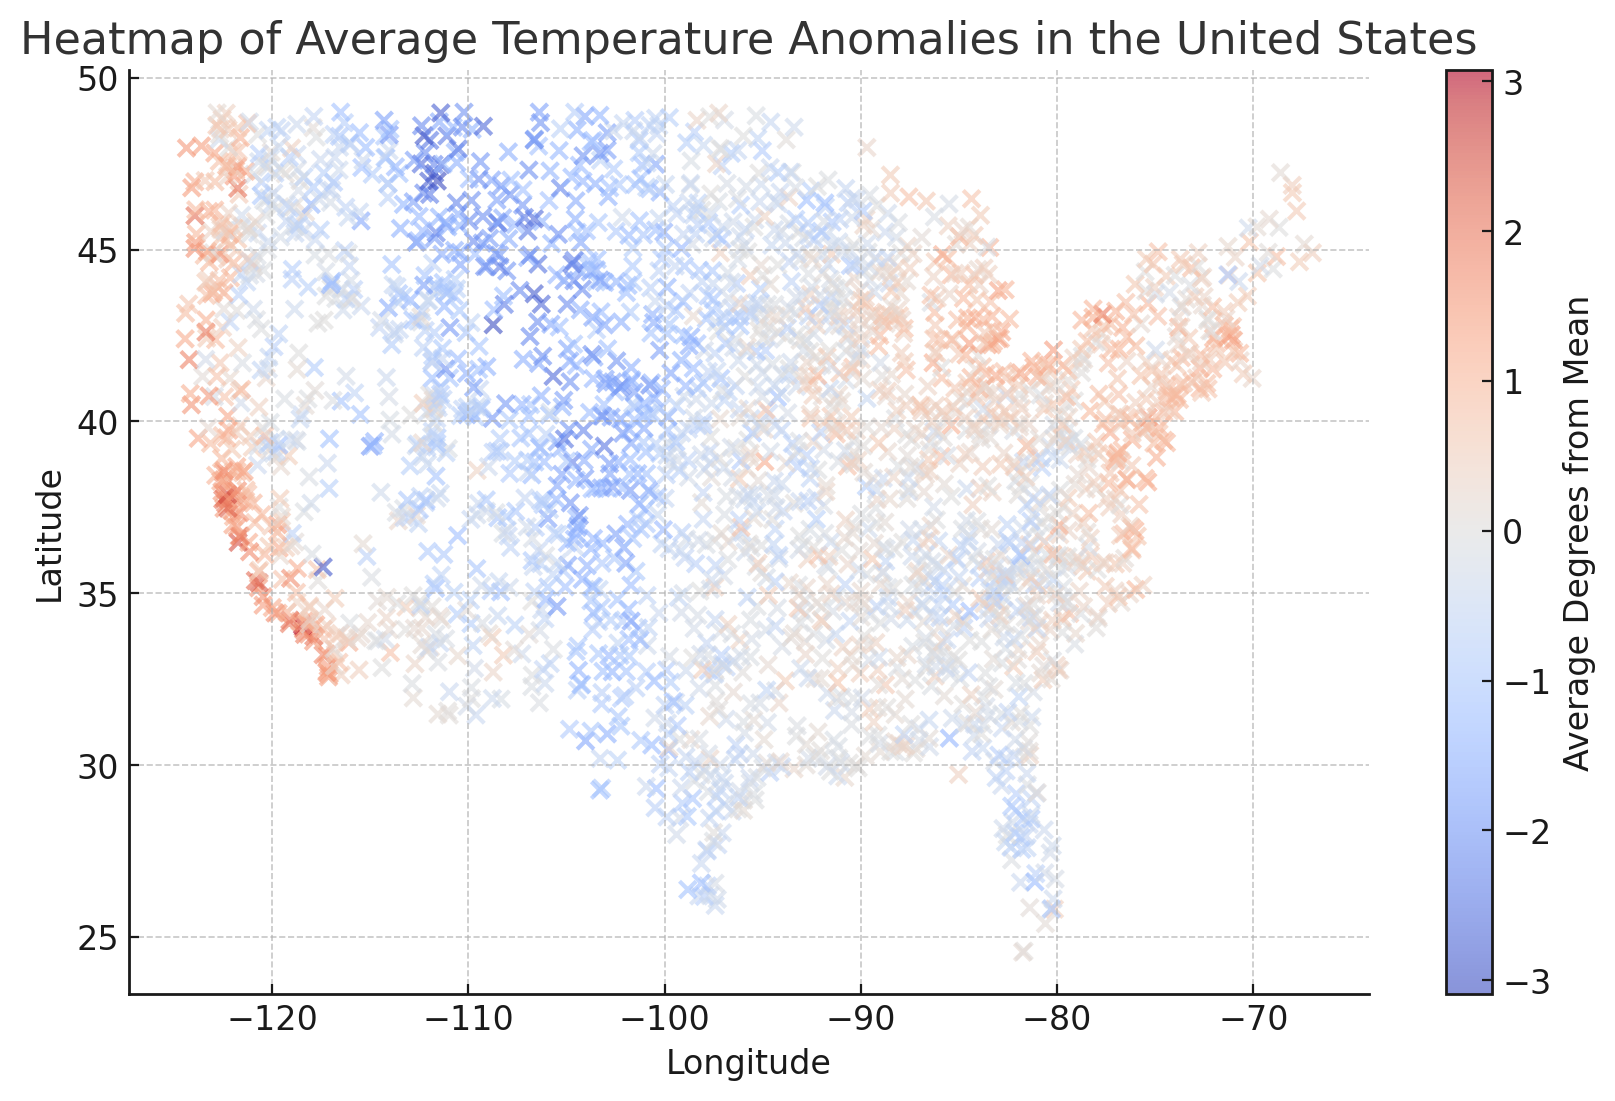
\includegraphics[width=\textwidth]{visuals/weather_visuals/Heat_map_USA.png}
    \caption{Heatmap of Average Temperature Anomalies in the United States}
    \label{fig:heatmap_usa}
\end{figure}


\subsubsection{Weather Data 1}

\subsection{Modelling wind speed from Large Weahter Data}

The wind data analyzed in this study originates from 54 stations located near Santa Barbara, California, USA. Data collection began in 1981 and has been ongoing, with contributions from three agencies: Santa Barbara County Air Pollution Control District, California Department of Water Resources, and National Data Buoy Center. Notably, the dataset also includes water temperature data from the National Data Buoy Center. This comprehensive dataset is updated annually, providing a valuable resource for longitudinal wind studies.

\subsubsection*{Dataset 2}

Observations in this dataset are recorded on an hourly basis and encompass various wind-related measurements. Key variables include:

\begin{itemize}
    \item \textbf{spd:} Wind speed, recorded in meters per second.
    \item \textbf{U:} Easterly component of wind velocity, in meters per second.
    \item \textbf{V:} Northerly component of wind velocity, in meters per second.
    \item \textbf{Utau:} 10-meter U wind stress, measured in pascals.
    \item \textbf{Vtau:} 10-meter V wind stress, also in pascals.
\end{itemize}

Wind stress (\(\tau\)) is calculated using the formula \(\tau_o = C_D \cdot \rho \cdot V_{10}^2\), where \(C_D\) represents the drag coefficient, \(\rho\) the density of air, and \(V_{10}\) the wind speed at a height of 10 meters.
\newline

To enhance the analysis, the following engineered variables were created:
\begin{itemize}
    \item \textbf{spd\_rolling\_average:} A 7-day rolling average of wind speed (spd).
    \item \textbf{residuals\_sarima:} Residuals derived from an auto.arima model fitted on spd, with parameters set as frequency = 24, seasonal = TRUE, and approximation = FALSE.
\end{itemize}


For the analysis, the dataset was filtered to include observations from September 1, 2007, to October 18, 2007, a period marked by higher-than-usual wind speeds. The data underwent rigorous cleaning to address missing values and remove unnatural spd outliers. Missing values in Utau and Vtau were imputed using interpolation (forecast::na.interp).
\newline

A spline regression model was fitted to predict wind speeds (spd), with the following formula:
\begin{equation}
    spd \sim s(U) + s(V) + s(Utau) + s(Vtau) + s(residuals\_sarima) + s(spd\_rolling\_avg), \quad family = gaussian(link = "identity")
\end{equation}

This model selection reflects a focus on capturing both linear and non-linear relationships within the wind data, providing a robust framework for understanding wind speed dynamics in the region.

\newpage












\section{Appendix}



\bibliographystyle{unsrt}
\bibliography{References}

\end{document}
